\documentclass[11pt]{article} % use larger type; default would be 10pt

\usepackage{tikz}
\usepackage{pgfplots}
\usetikzlibrary{calc}
\usetikzlibrary{arrows}
\usetikzlibrary{patterns}
        \newcommand\degree[0]{^{\circ}}

\title{Play with TikZ}
\author{Just Us}
%\date{} % Activate to display a given date or no date (if empty),
         % otherwise the current date is printed 

\begin{document}
\maketitle

\section{Chap 4 Trigonometric Functions}

exam4-1-1
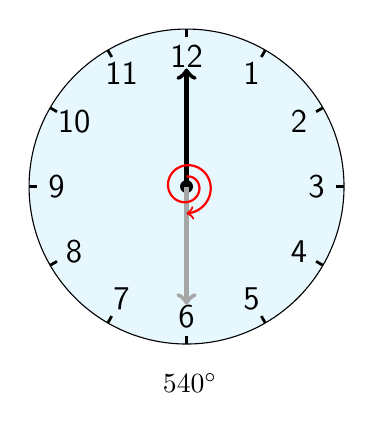
\begin{tikzpicture}
\coordinate(O) at (0,0);
\filldraw [fill=cyan!10!white] (O) circle [radius=2cm];
\filldraw [black] (O) circle [radius=.075cm];
\foreach \angle [count=\xi] in {60,30,...,-270}
{
  \draw[line width=1pt] (\angle:1.9cm) -- (\angle:2cm);
  \node[font=\large] at (\angle:1.65cm) {\textsf{\xi}};
}
\draw[black,ultra thick,->] (O) -- (90:1.5cm);
\draw[gray!70!white,ultra thick,->] (0,0) -- (270:1.5cm);

\draw [thick, color=red, ->, domain=9*pi/2:3*pi/2, samples=200, smooth]
  plot (xy polar cs:angle=\x r, radius={.45-(\x r)/2500});

\node[text width=.6cm] at (0,-2.5)  {$540\degree$};

\end{tikzpicture}
\newline


exam4-1-1b
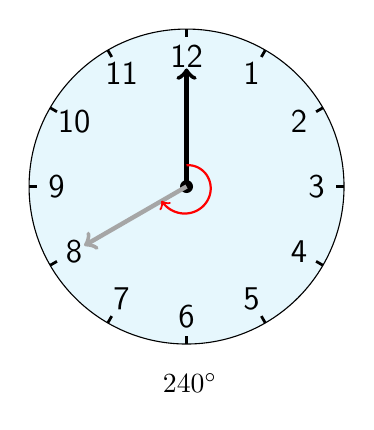
\begin{tikzpicture}
\coordinate(O) at (0,0);
\filldraw [fill=cyan!10!white] (O) circle [radius=2cm];
\filldraw [black] (O) circle [radius=.075cm];
\foreach \angle [count=\xi] in {60,30,...,-270}
{
  \draw[line width=1pt] (\angle:1.9cm) -- (\angle:2cm);
  \node[font=\large] at (\angle:1.65cm) {\textsf{\xi}};
}
\draw[black,ultra thick,->] (O) -- (90:1.5cm);
\draw[gray!70!white,ultra thick,->] (0,0) -- (210:1.5cm);

\draw [thick, color=red, ->, domain=5*pi/2:7*pi/6, samples=200, smooth]
  plot (xy polar cs:angle=\x r, radius={.45-(\x r)/2500});

\node[text width=.6cm] at (0,-2.5)  {$240\degree$};

\end{tikzpicture}
\newline


exer4-1-1
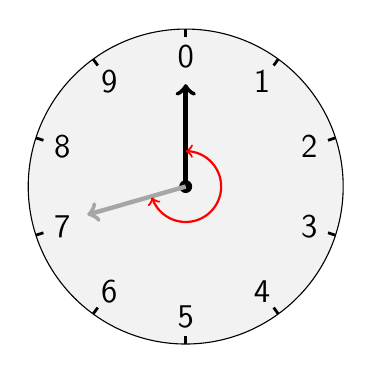
\begin{tikzpicture} 
\coordinate(O) at (0,0);
\filldraw [fill=gray!10!white] (O) circle [radius=2cm];
\filldraw [black] (O) circle [radius=.075cm];
\foreach 	[evaluate={\xmod=int(mod(\xi+1,10));}]
 \angle [count=\xi] in {54,18,...,-270}
{
  \draw[line width=1pt] (\angle:1.9cm) -- (\angle:2cm);
  \node[font=\large] at (\angle:1.65cm) {\textsf{\xmod}};
}
\draw[black,ultra thick,->] (O) -- (90:1.3cm);
\draw[gray!70!white,ultra thick,->] (0,0) -- (196:1.3cm);

\draw [thick, color=red, <->, domain=pi/2:-9*pi/10, samples=200, smooth]
  plot (xy polar cs:angle=\x r, radius={.45});

\end{tikzpicture}
\newline


fig-4-1-angles320
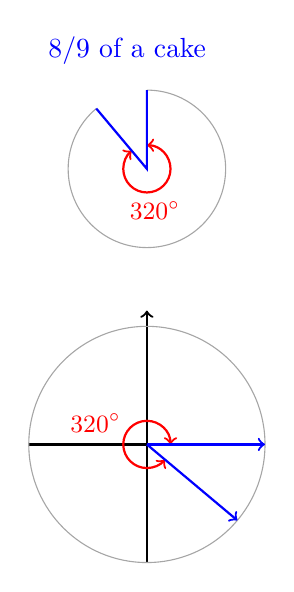
\begin{tikzpicture} 
\coordinate(O) at (0,0);
\coordinate(A) at (0,1);
\coordinate(B) at (130:1);

\draw [thick, color=red, <->] (0,.3) arc(90:-230:.3) node[below, midway] {\small$320\degree$};
\draw[gray!70!white] (0,1) arc(90:-230:1);
\draw[blue,thick] (A)--(O)--(B);

%second angle
\coordinate(O) at (0,-3.5);
\coordinate(A) at (1.5,-3.5);
\coordinate(B) at ($ (O)++1.5*cos(320)*(1,0) ++ 1.5*sin(320)*(0,1) $);

\draw[black,thick,->] (O)++(0,-1.5)--++(0,3.2);
\draw[black,thick] (O)--+(-1.5,0); 

\draw [thick, color=red, <->] (O)++(.3,0) arc(0:320:.3) node[above left, midway, inner sep=1pt] {\small$320\degree$};
\draw[gray!70!white] (O) circle(1.5);
\draw[blue,thick,<-] (A)--(O);
\draw[blue,thick,->] (O)--(B);

\node[text width=2.5cm] at (0,1.5) {\color{blue} 8/9 of a cake};

\end{tikzpicture}
\newline


fig-4-1-angles40minutes
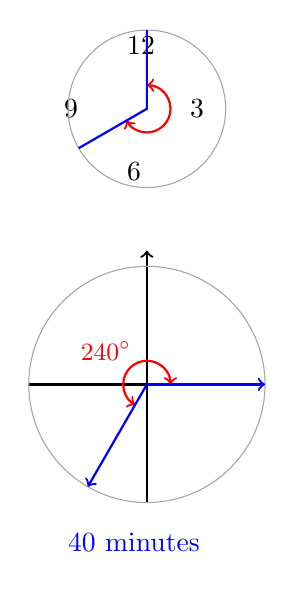
\begin{tikzpicture} 
\coordinate(O) at (0,0);
\coordinate(A) at (0,1);
\coordinate(B) at (210:1);
\node[text width=.5cm] at (0,.8) {12};
\node[text width=.5cm] at (0,-.8) {6};
\node[text width=.5cm] at (.8,0) {3};
\node[text width=.5cm] at (-.8,0) {9};


\draw [thick, color=red, <->] (0,.3) arc(90:-150:.3) ;
\draw[gray!70!white] (O) circle (1);
\draw[blue,thick] (A)--(O)--(B);

%second angle
\coordinate(O) at (0,-3.5);
\coordinate(A) at (1.5,-3.5);
\coordinate(B) at ($ (O)++1.5*cos(240)*(1,0) ++ 1.5*sin(240)*(0,1) $);

\draw[black,thick,->] (O)++(0,-1.5)--++(0,3.2);
\draw[black,thick] (O)--+(-1.5,0); 

\draw [thick, color=red, <->] (O)++(.3,0) arc(0:240:.3) node[above left, midway, inner sep=1pt] {\small$240\degree$};
\draw[gray!70!white] (O) circle(1.5);
\draw[blue,thick,<-] (A)--(O);
\draw[blue,thick,->] (O)--(B);

\node[text width=2.cm] at (0,-5.5) {\color{blue} 40 minutes};

\end{tikzpicture}
\newline


fig-4-1-angles-relativedirection
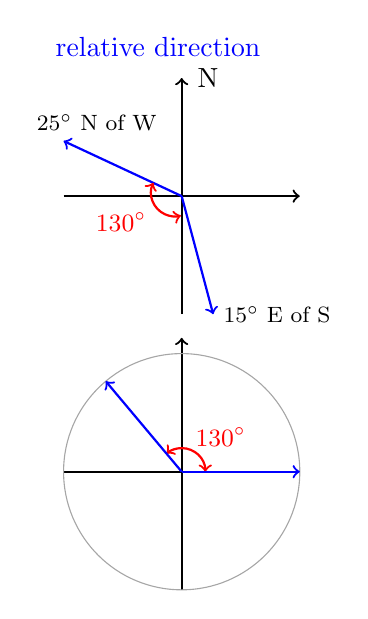
\begin{tikzpicture} 
\coordinate(O) at (0,0);
\coordinate(A) at (-1.5,0.7);
\coordinate(B) at (.4,-1.5);

\draw[black,thick,->] (-1.5,0)--(1.5,0);
\draw[black,thick,->] (0,-1.5)--(0,1.5) node[right, xshift=2] {N};

\draw [thick, color=blue, ->] (O)--(A) node[above, xshift=12] {\footnotesize\color{black} $25\degree$ N of W} ;
\draw [thick, color=blue, ->] (O)--(B) node[right] {\footnotesize\color{black} $15\degree$ E of S} ;

\draw[red,thick,<->] (O)++(-.36,.169) arc(155:285:.3) node[left,midway, yshift=-5] {\small$130\degree$};

%second angle
\coordinate(O) at (0,-3.5);
\coordinate(A) at (1.5,-3.5);
\coordinate(B) at ($ (O)++1.5*cos(130)*(1,0) ++ 1.5*sin(130)*(0,1) $);

\draw[black,thick,->] (O)++(0,-1.5)--++(0,3.2);
\draw[black,thick] (O)--+(-1.5,0); 

\draw [thick, color=red, <->] (O)++(.3,0) arc(0:130:.3) node[above right, midway, inner sep=1pt] {\small$130\degree$};
\draw[gray!70!white] (O) circle(1.5);
\draw[blue,thick,<-] (A)--(O);
\draw[blue,thick,->] (O)--(B);

\node[text width=3.2cm] at (0,1.9) {\color{blue} relative direction};

\end{tikzpicture}
\newline


fig-4-1-angles-difference-of-angles
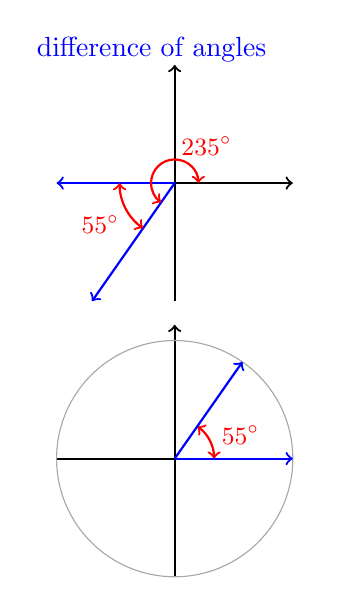
\begin{tikzpicture} 
\coordinate(O) at (0,0);
\coordinate(A) at (-1.5,0);
\coordinate(B) at (-1.05,-1.5);

\draw[black,thick,->] (-1.5,0)--(1.5,0);
\draw[black,thick,->] (0,-1.5)--(0,1.5);

\draw [thick, color=blue, ->] (O)--(A);
\draw [thick, color=blue, ->] (O)--(B);

\draw[red,thick,<->] (O)++(-0.7,0) arc(180:235:.7) node[below left,midway, inner sep=2pt] {\small$55\degree$};
\draw[red,thick,<->] (O)++(0.3,0) arc(0:235:.3) node[above right,midway, inner sep=2pt, xshift=4] {\small$235\degree$};

%second angle
\coordinate(O) at (0,-3.5);
\coordinate(A) at (1.5,-3.5);
\coordinate(B) at ($ (O)++1.5*cos(55)*(1,0) ++ 1.5*sin(55)*(0,1) $);

\draw[black,thick,->] (O)++(0,-1.5)--++(0,3.2);
\draw[black,thick] (O)--+(-1.5,0); 

\draw [thick, color=red, <->] (O)++(.5,0) arc(0:55:.5) node[right, midway, yshift=2, inner sep=4pt] {\small$55\degree$};
\draw[gray!70!white] (O) circle(1.5);
\draw[blue,thick,<-] (A)--(O);
\draw[blue,thick,->] (O)--(B);

\node[text width=3.5cm] at (0,1.7) {\color{blue} difference of angles};

\end{tikzpicture}
\newline


exam4-1-2a
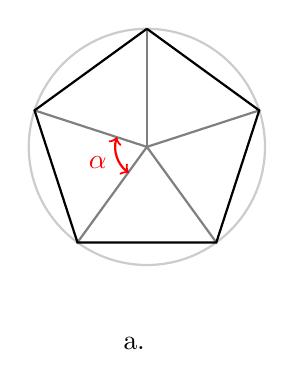
\begin{tikzpicture}
\coordinate(O) at (0,0);
\coordinate(A) at (90:1.5cm);
\coordinate(B) at (18:1.5cm);
\coordinate(C) at (-54:1.5cm);
\coordinate(D) at (-126:1.5cm);
\coordinate(E) at (-198:1.5cm);
\draw [gray!40!white,thick] (O) circle [radius=1.5cm];
\foreach [evaluate={\angleB=\xi*(-72)+90;}] \angle [count=\xi]  in {90,18,...,-270}
{
  \draw[gray,thick] (O) -- (\angle:1.5cm);
}

\draw[black,thick] (A)--(B)--(C)--(D)--(E)--(A);

\draw [red,thick,<->] ($.4*cos(162)*(1,0)++.4*sin(162)*(0,1) $) arc(162:235:0.4) node[left,midway, yshift=-2] {$\alpha$};

\node[text width=.6cm] at (0,-2.5)  {a.};

\end{tikzpicture}
\newline


exam4-1-2b
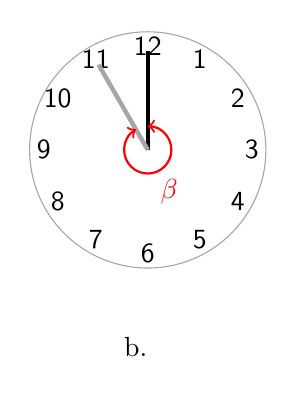
\begin{tikzpicture} 
\coordinate(O) at (0,0);
\draw [gray!70!white] (O) circle [radius=1.5cm];
\foreach \angle [count=\xi] in {60,30,...,-270}
{
  \node at (\angle:1.32cm) {\textsf{\xi}};
}
\draw[black,ultra thick] (O) -- (90:1.25cm);
\draw[gray!70!white,ultra thick] (0,0) -- (120:1.25cm);

\draw [red,thick, <->] (0,.3) arc(90:-240:.3) node[below right, midway, inner sep=2pt] {$\beta$};

\node[text width=.6cm] at (0,-2.5)  {b.};

\end{tikzpicture}
\newline


exam4-1-2aans
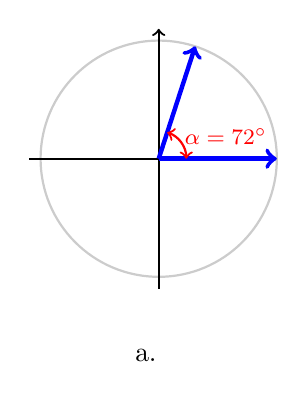
\begin{tikzpicture}
\coordinate(O) at (0,0);
\coordinate(A) at (0:1.5cm);
\coordinate(B) at (72:1.5cm);

\draw [gray!40!white,thick] (O) circle [radius=1.5cm];
\draw[black, thick,->] (0,-1.65)--(0,1.65);
\draw[black, thick] (O)--++(-1.65,0);
\draw[blue, ultra thick,->] (O)--(A);
\draw[blue, ultra thick,->] (O)--(B);

\draw [red,thick,<->] (0.35,0) arc(0:72:0.35) node[above right,midway, yshift=-2, inner sep=1pt] {\footnotesize $\alpha=72\degree$};

\node[text width=.6cm] at (0,-2.5)  {a.};

\end{tikzpicture}
\newline


exam4-1-2bans
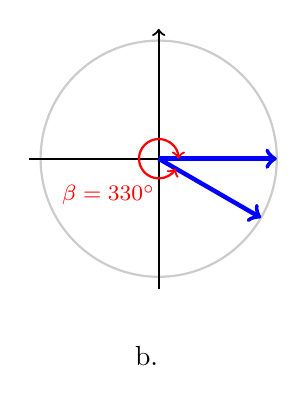
\begin{tikzpicture}
\coordinate(O) at (0,0);
\coordinate(A) at (0:1.5cm);
\coordinate(B) at (330:1.5cm);

\draw [gray!40!white,thick] (O) circle [radius=1.5cm];
\draw[black, thick,->] (0,-1.65)--(0,1.65);
\draw[black, thick] (O)--++(-1.65,0);
\draw[blue, ultra thick,->] (O)--(A);
\draw[blue, ultra thick,->] (O)--(B);

\draw [red,thick,<->] (0.25,0) arc(0:330:0.25) node[below left,midway, xshift=7, yshift=-10, inner sep=1pt] {\footnotesize $\beta=330\degree$};

\node[text width=.6cm] at (0,-2.5)  {b.};

\end{tikzpicture}
\newline


exer4-1-2a
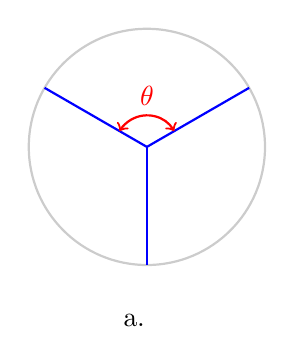
\begin{tikzpicture}
\coordinate(O) at (0,0);
\draw [gray!40!white,thick] (O) circle [radius=1.5cm];
\foreach \angle in {30,150,270}
{
  \draw[blue,thick] (O) -- (\angle:1.5cm);
}

\draw [red,thick,<->] ($.4*cos(30)*(1,0)++.4*sin(30)*(0,1) $) arc(30:150:0.4) node[above,midway] {$\theta$};

\node[text width=.6cm] at (0,-2.2)  {a.};

\end{tikzpicture}
\newline


exer4-1-2b
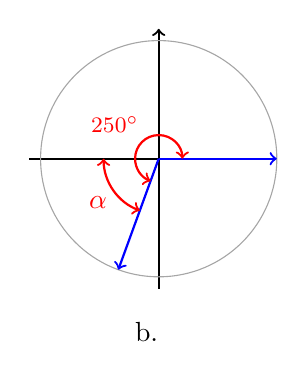
\begin{tikzpicture} 
\coordinate(O) at (0,0);
\coordinate(A) at (0:1.5cm);
\coordinate(B) at (250:1.5cm);

\draw[black, thick,->] (0,-1.65)--(0,1.65);
\draw[black, thick] (O)--++(-1.65,0);
\draw [gray!70!white] (O) circle [radius=1.5cm];

\draw[blue, thick,->] (O) -- (A);
\draw[blue, thick,->] (O) -- (B);

\draw [red,thick, <->] (.3,0) arc(0:250:.3) node[above left, midway, inner sep=2pt] {\footnotesize $250\degree$};
\draw [red,thick, <->] (-.7,0) arc(180:250:.7) node[below left, midway, inner sep=2pt] {$\alpha$};

\node[text width=.6cm] at (0,-2.2)  {b.};

\end{tikzpicture}
\newline


fig-4-1stanpos
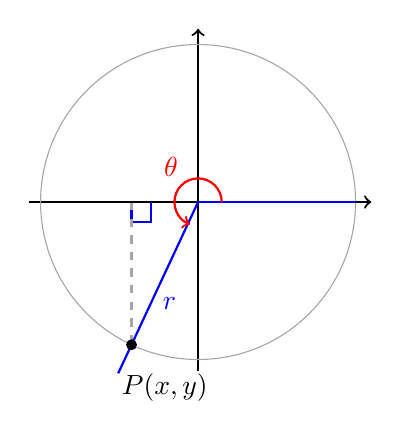
\begin{tikzpicture} 
\coordinate(O) at (0,0);
\coordinate(A) at (0:2cm);
\coordinate(B) at (245:2cm);
\coordinate(C) at ($ 2*cos(245)*(1,0) $);

\draw[blue, thick] (C) rectangle +(.25,-.25);
\draw[gray!70!white, thick, dashed] (C) -- (B);

\draw[black, thick,->] (0,-2.15)--(0,2.2);
\draw[black, thick, ->] (-2.15,0)--(2.2,0);
\draw [gray!70!white] (O) circle [radius=2cm];

\draw[blue, thick] (O) -- (A);
\draw[blue, thick] (O) -- ($ 2.4*cos(245)*(1,0)++2.4*sin(245)*(0,1) $) node[below right, midway, xshift=-2] {$r$};

\draw [red,thick, ->] (.3,0) arc(0:250:.3) node[above left, midway, inner sep=2pt] {$\theta$};

\filldraw[black] (B) circle (1.75pt) node[anchor=north west, xshift=-7, yshift=-7] {$P(x,y)$};

\end{tikzpicture}
\newline


exam4-1-3a
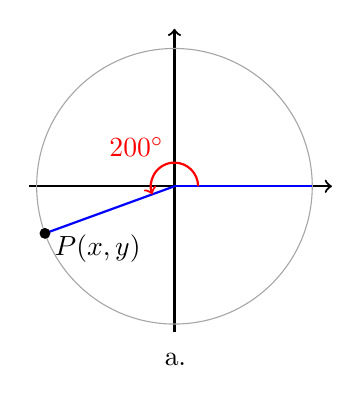
\begin{tikzpicture} 
\coordinate(O) at (0,0);
\coordinate(A) at (0:1.75cm);
\coordinate(B) at (200:1.75cm);

\draw[black, thick,->] (0,-1.85)--(0,2);
\draw[black, thick, ->] (-1.85,0)--(2,0);
\draw [gray!70!white] (O) circle [radius=1.75cm];

\draw[blue, thick] (O) -- (A);
\draw[blue, thick] (O) -- (B);

\draw [red,thick, ->] (O)++(.3,0) arc(0:200:.3) node[above left, midway, inner sep=2pt] {$200\degree$};

\filldraw[black] (B) circle (1.75pt) node[anchor=north west, xshift=0, yshift=3] {$P(x,y)$};

\node[text width=.25cm] at (0,-2.2)  {a.};

\end{tikzpicture}
\newline


exam4-1-3b
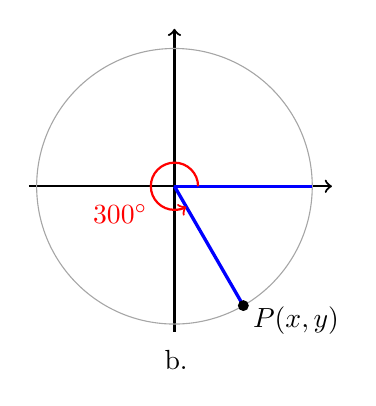
\begin{tikzpicture} 
\coordinate(O) at (0,0);
\coordinate(A) at (0:1.75cm);
\coordinate(B) at (300:1.75cm);

\draw[black, thick,->] (0,-1.85)--(0,2);
\draw[black, thick, ->] (-1.85,0)--(2,0);
\draw [gray!70!white] (O) circle [radius=1.75cm];

\draw[blue, very thick] (O) -- (A);
\draw[blue, very thick] (O) -- (B);

\draw [red,thick, ->] (O)++(.3,0) arc(0:300:.3) node[below left, yshift=-.3cm, midway, inner sep=2pt] {$300\degree$};

\filldraw[black] (B) circle (1.75pt) node[anchor=north west, xshift=0, yshift=3] {$P(x,y)$};

\node[text width=.25cm] at (0,-2.2)  {b.};

\end{tikzpicture}
\newline

exam4-1-4
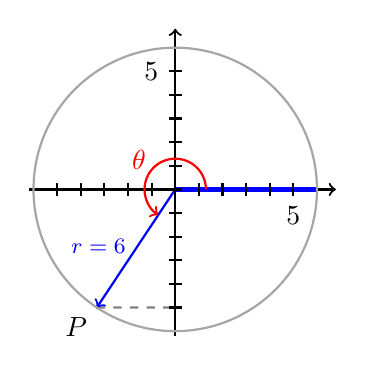
\begin{tikzpicture}[scale=.3]
\coordinate(O) at (0,0);
\coordinate(A) at (0:6);
%\coordinate(B) at ($ -6*asin(5/6)*(1,0)++(0,-5)$);
\coordinate(B) at (-3.32,-5);

\draw[thick,->] (-6.2,0) -- (6.8,0);
\draw[thick,->] (0,-6.2) -- (0,6.8);
\draw[gray,thick,dashed] (B) -- (0,-5);
\draw[blue, ultra thick] (O) -- (A);
\draw[blue,  thick, ->] (O) -- (B) node[above left, midway, yshift=-.2cm] {\footnotesize $r=6$};

\foreach \x in {-5,-4,...,4}
    \draw[black,thick] (\x cm,8pt) -- (\x cm,-8pt) ;
\foreach \y in {-5,-4,...,4}
    \draw[black,thick] (8pt,\y cm) -- (-8pt,\y cm);
\draw[black,thick] (5 cm,8pt) --(5cm,-8pt) node[anchor=north] {$5$};     		
\draw[black,thick] (8pt,5 cm) -- (-8pt,5 cm) node[anchor=east] {$5$};

\filldraw[black] (B) circle (.75pt) node[anchor=north east, xshift=0, yshift=0] {$P$};
\draw[gray!70!white,thick] (O) circle (6cm);

\draw [red,thick, ->] (O)++(1.3,0) arc(0:{180+asin(5/6)}:1.3) node[above left, xshift=-3, yshift=-5, midway, inner sep=2pt] {$\theta$};

\end{tikzpicture}
\newline

exer4-1-4
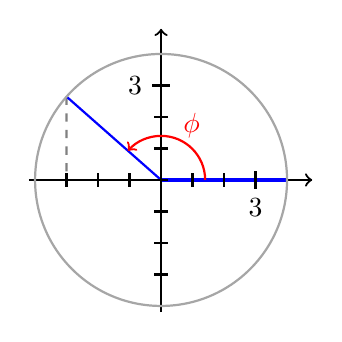
\begin{tikzpicture}[scale=.4]
\coordinate(O) at (0,0);
\coordinate(A) at (0:4);
%\coordinate(B) at ($ -6*asin(5/6)*(1,0)++(0,-5)$);
\coordinate(B) at (138.6:4);
\draw[gray,thick,dashed] (B) -- (-3,0);

\draw[thick,->] (-4.2,0) -- (4.8,0);
\draw[thick,->] (0,-4.2) -- (0,4.8);
\draw[blue, ultra thick] (O) -- (A);
\draw[blue,  thick ] (O) -- (B) ;

\foreach \x in {-3,-2,...,3}
    \draw[black,thick] (\x cm,6pt) -- (\x cm,-6pt) ;
\foreach \y in {-3,-2,...,3}
    \draw[black,thick] (6pt,\y cm) -- (-6pt,\y cm);
\draw[black,thick] (3 cm,8pt) --(3cm,-8pt) node[anchor=north] {$3$};     		
\draw[black,thick] (8pt,3 cm) -- (-8pt,3 cm) node[anchor=east] {$3$};
\draw[gray!70!white,thick] (O) circle (4cm);

\draw [red,thick, ->] (O)++(1.4,0) arc(0:{acos(-3/4)}:1.4) node[above right, xshift=-0, yshift=-2, midway, inner sep=2pt] {$\phi$};

\end{tikzpicture}
\newline


fig-4-1-refang
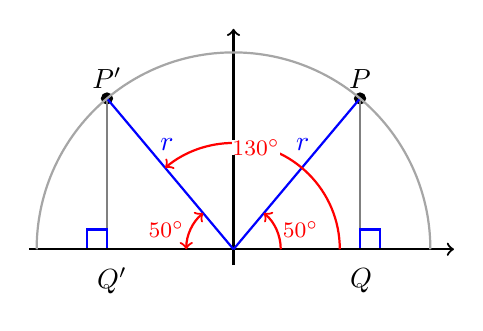
\begin{tikzpicture} 
\coordinate(O) at (0,0);
\coordinate(P) at (50:2.5);
\filldraw (P) circle (2pt) node[anchor=south]{$P$};
\node[text width=.25cm] at ($ 2.5*cos(50)*(1,0) + (0,-.4)  $) {$Q$};

\draw[gray,thick] (P) -- +($ -2.5*sin(50)*(0,1) $);
\draw[blue,thick] ($ 2.5*cos(50)*(1,0) $) rectangle +(.25,.25);
\coordinate(Pp) at (130:2.5);
\filldraw (Pp) circle (2pt) node[anchor=south]{$P'$};
\node[text width=.25cm] at ($ -2.5*cos(50)*(1,0) + (0,-.4)  $) {$Q'$};
\draw[gray,thick] (Pp) -- +($ -2.5*sin(50)*(0,1) $);
\draw[blue,thick] ($ -2.5*cos(50)*(1,0) $) rectangle +(-.25,.25);

\draw[thick,->] (-2.6,0) -- (2.8,0);
\draw[thick,->] (0,-.2) -- (0,2.8);
\draw[blue, thick] (O) -- (P) node[above left, midway, xshift=6, yshift=7, inner sep=1pt] {$r$};
\draw[blue, thick ] (O) -- (Pp) node[above right, xshift=-5, yshift=7, midway, inner sep=1pt] {$r$} ;

\draw[gray!70!white,thick] (O)++(2.5,0) arc (0:180:2.5cm);

\draw [red,thick, ->] (O)++(.6,0) arc(0:50:.6) node[ right, xshift=-0, yshift=0, midway, inner sep=2pt] {\footnotesize$50\degree$};

\draw [red,thick, ->] (O)++(1.35,0) arc(0:130:1.35) node[ right, xshift=-0, yshift=0, midway, xshift=-17, yshift=2, fill=white,inner sep=0pt] {\footnotesize$130\degree$};

\draw [red,thick, <->] (O)++(-.6,0) arc(180:130:.6) node[ left, xshift=-0, yshift=0, midway, inner sep=2pt] {\footnotesize$50\degree$};
\end{tikzpicture}
\newline

fig-4-1ref
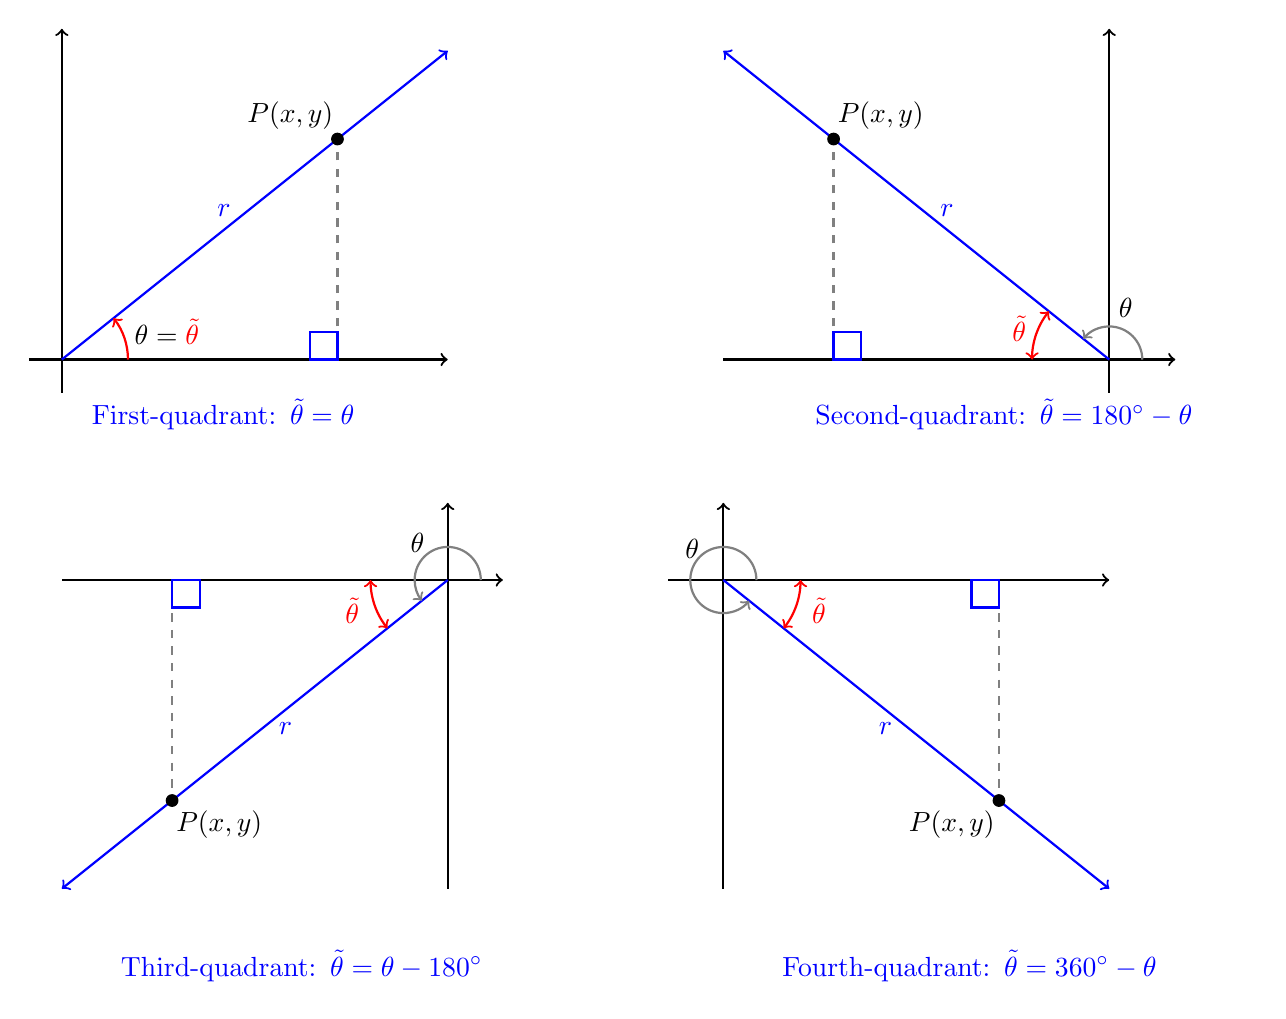
\begin{tikzpicture}[scale=1.4]

\coordinate (O) at (0,0);
\coordinate (x) at (2.5,0);
\coordinate (P) at (2.5,2);
\coordinate (A) at (3.5,0);
\coordinate (B) at (0,3);
\coordinate (C) at (3.5,2.8);

\draw[black,  thick, ->] (O)++(-.3,0) --(A);
\draw[black,  thick, ->] (O)++(0,-.3) -- (B) ;
\draw[blue,  thick, ->] (O) --  (C) node[left, midway, xshift=-5, yshift=-2]{$r$}  ;
\draw[red, thick, ->] (.6,0) arc (0:{atan(2/2.5)}:.6) node [right, midway,xshift=0,yshift=2] {$\color{black}\theta=\color{red}\tilde{\theta}$};

\draw[gray, thick, dashed] (x) -- (P);
\draw[blue, thick] (x) rectangle +(-.25,.25);

\filldraw (P) circle (1.5pt) node[anchor = south east, xshift=2]{$P(x,y)$}; 

\node[text width=4cm] at (1.7,-.5)     {\color{blue} First-quadrant: $\tilde{\theta}=\theta$};

%second quadrant


\coordinate (O) at (9.5,0);
\coordinate (x) at (7,0);
\coordinate (P) at (7,2);
\coordinate (A) at (6,0);
\coordinate (B) at (9.5,3);
\coordinate (C) at (6,2.8);

\draw[black,  thick, <-] (O)++(.6,0) --(A);
\draw[black,  thick, ->] (O)++(0,-.3) -- (B) ;
\draw[blue,  thick, ->] (O) --  (C) node[right, midway, xshift=5, yshift=-2]{$r$}  ;

\draw[red, thick, <->] (O)++(-.7,0) arc (180:{180-atan(2/2.5)}:.7) node [left, midway,xshift=0,yshift=2] {$\tilde{\theta}$};
\draw[gray, thick, ->] (O)++(.3,0) arc (0:{180-atan(2/2.5)}:.3) node [above, midway,xshift=2,yshift=0] {\color{black}$\theta$};

\draw[gray, thick, dashed] (x) -- (P);
\draw[blue, thick] (x) rectangle +(.25,.25);

\filldraw (P) circle (1.5pt) node[anchor = south west, xshift=-2]{$P(x,y)$}; 

\node[text width=5.5cm] at (8.8,-.5)     {\color{blue} Second-quadrant: $\tilde{\theta}=180\degree-\theta$};

%third quadrant

\coordinate (O) at (3.5,-2);
\coordinate (x) at (1,-2);
\coordinate (P) at (1,-4);
\coordinate (A) at (0,-2);
\coordinate (B) at (3.5,-4.8);
\coordinate (C) at (0,-4.8);

\draw[black,  thick, <-] (O)++(.5,0) --(A);
\draw[black,  thick, <-] (O)++(0,.7) -- (B) ;
\draw[blue,  thick, ->] (O) --  (C) node[right, midway, xshift=5, yshift=2]{$r$}  ;
\draw[red, thick, <->] (O)++(-.7,0) arc (180:{180+atan(2/2.5)}:.7) node [left, midway,xshift=-2,yshift=-2] {$\tilde{\theta}$};
\draw[gray, thick, ->] (O)++(.3,0) arc (0:{180+atan(2/2.5)}:.3) node [above, midway,xshift=-7,yshift=-5] {\color{black}$\theta$};

\draw[gray, thick, dashed] (x) -- (P);
\draw[blue, thick] (x) rectangle +(.25,-.25);

\filldraw (P) circle (1.5pt) node[anchor = north west, xshift=-2]{$P(x,y)$}; 

\node[text width=5.5cm] at (2.5,-5.5)     {\color{blue} Third-quadrant: $\tilde{\theta}=\theta-180\degree$};

%fourth quadrant

\coordinate (O) at (6,-2);
\coordinate (x) at (8.5,-2);
\coordinate (P) at (8.5,-4);
\coordinate (A) at (9.5,-2);
\coordinate (B) at (6,-4.8);
\coordinate (C) at (9.5,-4.8);

\draw[black,  thick, ->] (O)++(-.5,0) --(A);
\draw[black,  thick, <-] (O)++(0,.7) -- (B) ;
\draw[blue,  thick, ->] (O) --  (C) node[left, midway, xshift=-5, yshift=2]{$r$}  ;
\draw[red, thick, <->] (O)++(.7,0) arc (0:{-atan(2/2.5)}:.7) node [right, midway,xshift=2,yshift=-2] {$\tilde{\theta}$};
\draw[gray, thick, ->] (O)++(.3,0) arc (0:{360-atan(2/2.5)}:.3) node [above, midway,xshift=0,yshift=0] {\color{black}$\theta$};

\draw[gray, thick, dashed] (x) -- (P);
\draw[blue, thick] (x) rectangle +(-.25,-.25);

\filldraw (P) circle (1.5pt) node[anchor = north east, xshift=2]{$P(x,y)$}; 

\node[text width=5.5cm] at (8.5,-5.5)     {\color{blue} Fourth-quadrant: $\tilde{\theta}=360\degree -\theta$};

\end{tikzpicture}
\newline


act4-1 grid

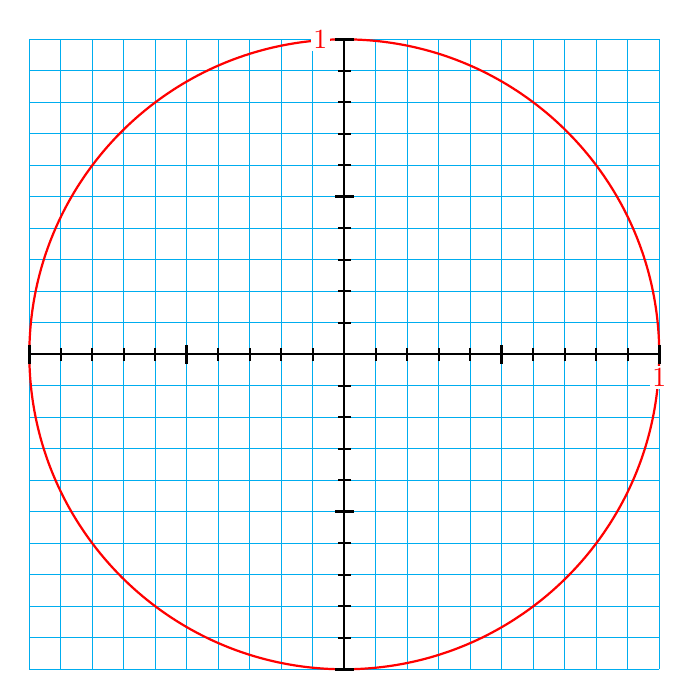
\begin{tikzpicture} [scale = .4] 
\draw[cyan] (-10,-10) grid (10,10);
\draw[black, thick] (-10,0) -- (10,0);
\draw[black, thick] (0,-10) -- (0, 10);

\coordinate (O) at (0,0);

\draw[red,thick] (O) circle (10cm);

\foreach \x  in {-10, -9, ..., 10} 
{
\draw[black,  thick] ($ \x *(1,0) +(0,.2) $) --++(0,-0.4); 
\draw[black,  thick] ($ \x *(0,1) +(.2,0) $) --++(-0.4,0); 
};

\foreach \x  in {-10, -5, 5, 10} 
{
\draw[black, very thick] ($ \x *(1,0) +(0,.3) $) --++(0,-0.6); 
\draw[black, very thick] ($ \x *(0,1) +(.3,0) $) --++(-0.6,0); 
};

\filldraw[black] (10,0) circle (.5pt) node[anchor=north, yshift=-4, fill=white, inner sep=1pt, text=red] {1};
\filldraw[black] (0,10) circle (.5pt) node[anchor=east, xshift=-5, fill=white, inner sep=1pt, text=red] {1};

\end{tikzpicture}
\newline


exam4-1-5
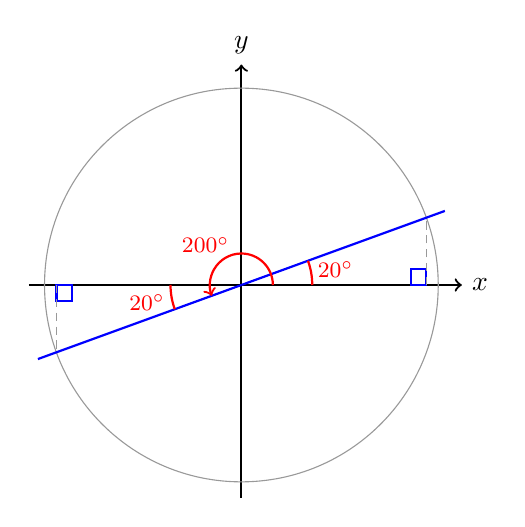
\begin{tikzpicture} 
\coordinate(O) at (0,0);
\coordinate(A) at (20:2.75cm);
\coordinate(B) at (200:2.75cm);

\draw[black, thick,->] (0,-2.7)--(0,2.8) node[above]{$y$};
\draw[black, thick, ->] (-2.7,0)--(2.8,0) node[right]{$x$};
\draw [gray!80!white] (O) circle [radius=2.5cm];

\draw[blue,thick] ($ 2.5*cos(20)*(1,0)$) rectangle +(-.2,.2);
\draw[gray!80!white, densely dashed] ($ 2.5*cos(20)*(1,0)$) --(20:2.5);
\draw[blue,thick] ($ 2.5*cos(20)*(-1,0)$) rectangle +(.2,-.2);
\draw[gray!80!white, densely dashed] ($ 2.5*cos(20)*(-1,0)$) --(200:2.5);

\draw[blue, thick] (O) -- (A);
\draw[blue, thick] (O) -- (B);

\draw [red,thick, ->] (O)++(.4,0) arc(0:200:.4) node[above left, midway, yshift=-2, inner sep=2pt] {\footnotesize$200\degree$};

\draw [red,thick] (O)++(.9,0) arc(0:20:.9) node[ right, midway, yshift=1, inner sep=2pt] {\footnotesize$20\degree$};
\draw [red,thick] (O)++(-.9,0) arc(180:200:.9) node[ left, midway, yshift=-2, inner sep=2pt] {\footnotesize$20\degree$};

\end{tikzpicture}
\newline


fig-4-1quads

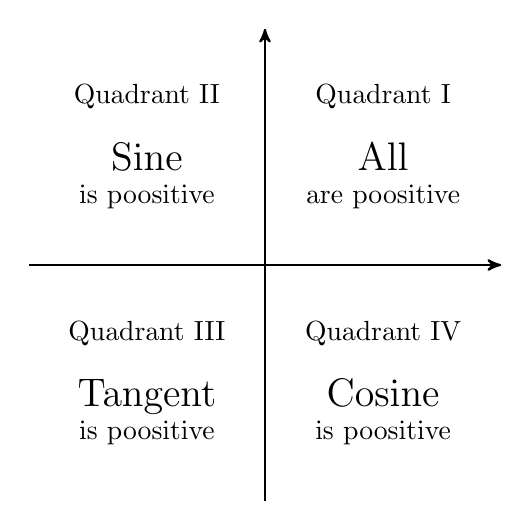
\begin{tikzpicture} 
\draw[black, thick,->,>=stealth'] (0,-3)--(0,3);
\draw[black, thick, ->,>=stealth'] (-3,0)--(3,0);

\node[align=center] at (1.5,1.5) {Quadrant I\\ \\ \Large{All}\\are poositive};
\node[align=center] at (-1.5,1.5) {Quadrant II\\ \\ \Large{Sine}\\is poositive};
\node[align=center] at (-1.5,-1.5) {Quadrant III\\ \\ \Large{Tangent}\\is poositive};
\node[align=center] at (1.5,-1.5) {Quadrant IV\\ \\ \Large{Cosine}\\is poositive};

\end{tikzpicture}
\newline


fig-4-1-bowtie
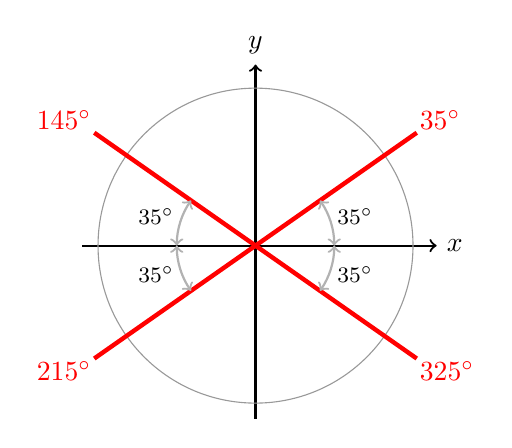
\begin{tikzpicture} 
\coordinate(O) at (0,0);
\coordinate(A) at (35:2.5cm);
\coordinate(B) at (215:2.5cm);
\coordinate(C) at (-35:2.5cm);
\coordinate(D) at (145:2.5cm);

\draw[black, thick,->] (0,-2.2)--(0,2.3) node[above]{$y$};
\draw[black, thick, ->] (-2.2,0)--(2.3,0) node[right]{$x$};
\draw [gray!80!white] (O) circle [radius=2cm];


\draw[red, ultra thick] (O) -- (A) node[above right, xshift=-3, yshift=-3] {$35\degree$};
\draw[red, ultra thick] (O) -- (B) node[below left, xshift=3, yshift=3] {$215\degree$};
\draw[red, ultra thick] (O) -- (D) node[above left, xshift=3, yshift=-3] {$145\degree$};
\draw[red, ultra thick] (O) -- (C) node[below right, xshift=-3, yshift=3] {$325\degree$};

\draw [gray!60!white,thick, <->] (O)++(1,0) arc(0:35:1) node[right, midway, yshift=2, inner sep=2pt] {\color{black}\footnotesize$35\degree$};

\draw [gray!60!white,thick, <->] (O)++(1,0) arc(0:-35:1) node[ right, midway, yshift=-2, inner sep=2pt] {\color{black}\footnotesize$35\degree$};
\draw [gray!60!white,thick, <->] (O)++(-1,0) arc(180:215:1) node[ left, midway, yshift=-2, inner sep=2pt] {\color{black}\footnotesize$35\degree$};
\draw [gray!60!white,thick, <->] (O)++(-1,0) arc(180:145:1) node[ left, midway, yshift=2, inner sep=2pt] {\color{black}\footnotesize$35\degree$};

\end{tikzpicture}
\newline


exam4-1-6a
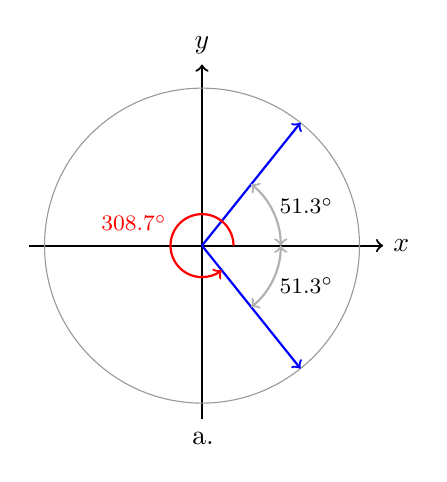
\begin{tikzpicture} 
\coordinate(O) at (0,0);
\coordinate(A) at (51.3:2cm);
\coordinate(B) at (-51.3:2cm);

\draw[black, thick,->] (0,-2.2)--(0,2.3) node[above]{$y$};
\draw[black, thick, ->] (-2.2,0)--(2.3,0) node[right]{$x$};
\draw [gray!80!white] (O) circle [radius=2cm];


\draw[blue, thick, ->] (O) -- (A);
\draw[blue, thick, ->] (O) -- (B);

\draw [gray!60!white,thick, <->] (O)++(1,0) arc(0:51.3:1) node[right, midway, yshift=2, inner sep=2pt] {\color{black}\footnotesize$51.3\degree$};

\draw [gray!60!white,thick, <->] (O)++(1,0) arc(0:-51.3:1) node[ right, midway, yshift=-2, inner sep=2pt] {\color{black}\footnotesize$51.3\degree$};
\draw [red,thick, ->] (O)++(.4,0) arc(0:308.7:.4) node[above left, midway, yshift=-2, inner sep=2pt] {\color{red}\footnotesize$308.7\degree$};

\node[text width=.25cm] at (0,-2.45){ a.};

\end{tikzpicture}
\newline



exam4-1-6b
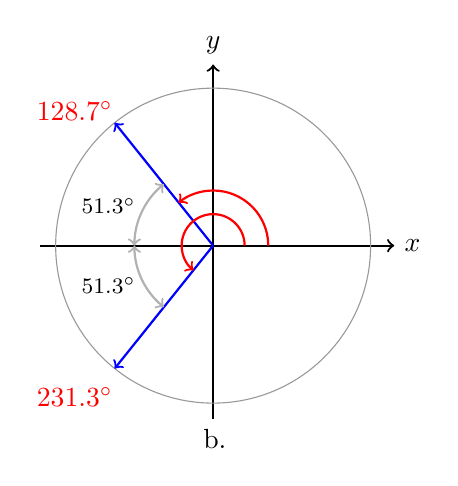
\begin{tikzpicture} 
\coordinate(O) at (0,0);
\coordinate(A) at (128.7:2cm);
\coordinate(B) at (231.3:2cm);

\draw[black, thick,->] (0,-2.2)--(0,2.3) node[above]{$y$};
\draw[black, thick, ->] (-2.2,0)--(2.3,0) node[right]{$x$};
\draw [gray!80!white] (O) circle [radius=2cm];


\draw[blue, thick, ->] (O) -- (A) node[above left, xshift=3, yshift=-3] {\color{red}$128.7\degree$};;
\draw[blue, thick, ->] (O) -- (B) node[below left, xshift=3, yshift=-3] {\color{red}$231.3\degree$};;

\draw [gray!60!white,thick, <->] (O)++(-1,0) arc(180:128.7:1) node[left, midway, yshift=2, inner sep=2pt] {\color{black}\footnotesize$51.3\degree$};

\draw [gray!60!white,thick, <->] (O)++(-1,0) arc(180:231.3:1) node[ left, midway, yshift=-2, inner sep=2pt] {\color{black}\footnotesize$51.3\degree$};
\draw [red,thick, ->] (O)++(.7,0) arc(0:128.7:.7);
\draw [red,thick, ->] (O)++(.4,0) arc(0:231.3:.4);

\node[text width=.25cm] at (0,-2.45){ b.};

\end{tikzpicture}
\newline



fig-4-1-coterm
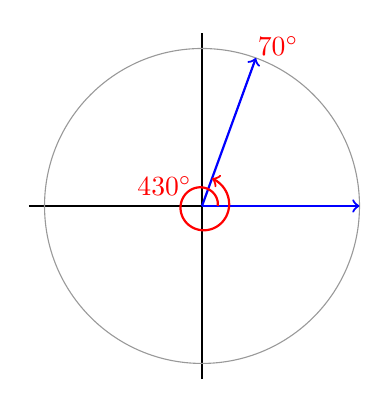
\begin{tikzpicture}
\coordinate(O) at (0,0);
\coordinate(A) at (70:2cm);
\draw[black, thick] (0,-2.2)--(0,2.2);
\draw[black, thick] (-2.2,0)--(0,0) ;
\draw [gray!80!white] (O) circle [radius=2cm];

\draw[blue, thick, ->] (O) -- +(2,0);
\draw[blue, thick, ->] (O) -- (A) node[above right, xshift=-3, yshift=-3] {\color{red}$70\degree$};

\draw [thick, color=red, ->, domain=0:pi*(2+7/18), samples=200, smooth]
  plot (xy polar cs:angle=\x r, radius={.2+(\x r)/2500}) node[above left, midway] {$430\degree$};

\end{tikzpicture}
\newline


fig-4-1-coterm2
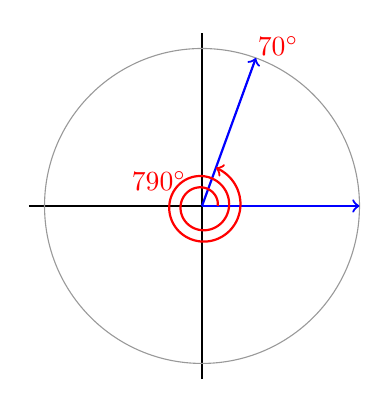
\begin{tikzpicture}
\coordinate(O) at (0,0);
\coordinate(A) at (70:2cm);
\draw[black, thick] (0,-2.2)--(0,2.2);
\draw[black, thick] (-2.2,0)--(0,0) ;
\draw [gray!80!white] (O) circle [radius=2cm];

\draw[blue, thick, ->] (O) -- +(2,0);
\draw[blue, thick, ->] (O) -- (A) node[above right, xshift=-3, yshift=-3] {\color{red}$70\degree$};

\draw [thick, color=red, ->, domain=0:pi*(4+7/18), samples=200, smooth]
  plot (xy polar cs:angle=\x r, radius={.2+(\x r)/2500}) node[above left, midway, xshift=-2, yshift=2] {$790\degree$};

\end{tikzpicture}
\newline


fig-4-1-negang
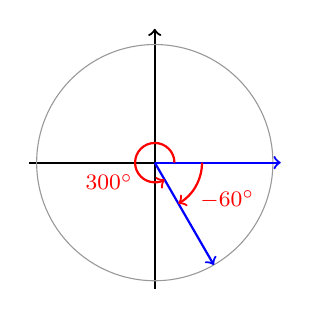
\begin{tikzpicture}
\coordinate(O) at (0,0);
\coordinate(A) at (-60:1.5cm);
\draw[black, thick, ->] (0,-1.6)--(0,1.7);
\draw[black, thick] (-1.6,0)--(0,0) ;
\draw [gray!80!white] (O) circle [radius=1.5];

\draw[blue, thick, ->] (O) -- +(1.6,0);
\draw[blue, thick, ->] (O) -- (A);

\draw [thick, color=red, ->](O)++(.25,0) arc (0:300:.25) node[below left, midway, xshift=2, yshift=-4] {\footnotesize$300\degree$};

\draw [thick, color=red, ->](O)++(.6,0) arc (0:-60:.6) node[below right, midway, xshift=-2, yshift=2] {\footnotesize$-60\degree$};

\end{tikzpicture}
\newline



fig-4-1-eqna
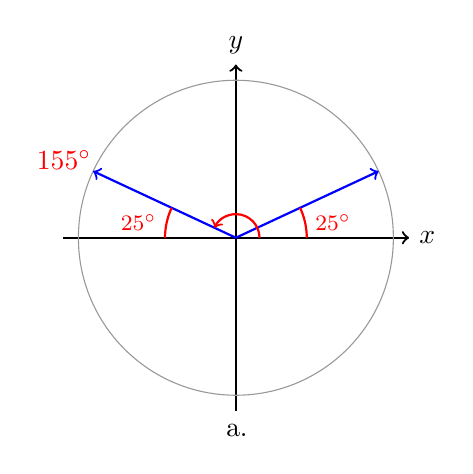
\begin{tikzpicture}
\coordinate(O) at (0,0);
\coordinate(A) at (25:2cm);
\coordinate(B) at (155:2cm);
\draw[black, thick, ->] (0,-2.2)--(0,2.2) node[above] {$y$};
\draw[black, thick, ->] (-2.2,0)--(2.2,0) node[right] {$x$};
\draw [gray!80!white] (O) circle [radius=2cm];

\draw[blue, thick, ->] (O) -- (B) node[above left, xshift=3, yshift=-3] {\color{red}$155\degree$};
\draw[blue, thick, ->] (O) -- (A);

\draw [thick, color=red] (O) ++(.9,0) arc(0:25:.9)
   node[right, midway] {\footnotesize$25\degree$};
\draw [thick, color=red] (O) ++(-.9,0) arc(180:155:.9)
   node[left, midway] {\footnotesize$25\degree$};
\draw [thick, red, ->] (O) ++(.3,0) arc(0:155:.3);

\node[text width=.25cm] at (0,-2.45){ a.};

\end{tikzpicture}
\newline


fig-4-1-eqnb
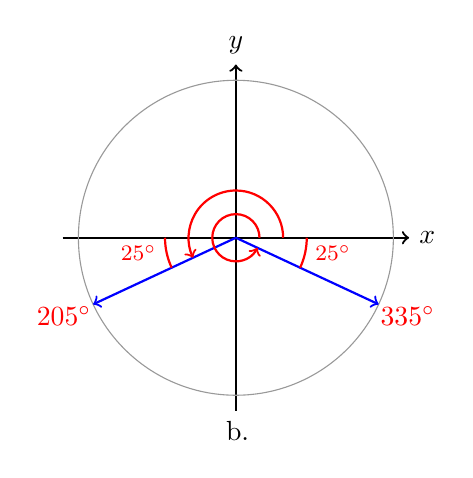
\begin{tikzpicture}
\coordinate(O) at (0,0);
\coordinate(A) at (-25:2cm);
\coordinate(B) at (205:2cm);
\draw[black, thick, ->] (0,-2.2)--(0,2.2) node[above] {$y$};
\draw[black, thick, ->] (-2.2,0)--(2.2,0) node[right] {$x$};
\draw [gray!80!white] (O) circle [radius=2cm];

\draw[blue, thick, ->] (O) -- (B) node[below left, xshift=3, yshift=3] {\color{red}$205\degree$};
\draw[blue, thick, ->] (O) -- (A) node[below right, xshift=-3, yshift=3] {\color{red}$335\degree$};

\draw [thick, color=red] (O) ++(.9,0) arc(0:-25:.9)
   node[right, midway] {\footnotesize$25\degree$};
\draw [thick, color=red] (O) ++(-.9,0) arc(180:205:.9)
   node[left, midway] {\footnotesize$25\degree$};
\draw [thick, red, ->] (O) ++(.3,0) arc(0:335:.3);
\draw [thick, red, ->] (O) ++(.6,0) arc(0:205:.6);

\node[text width=.25cm] at (0,-2.45){ b.};

\end{tikzpicture}
\newline


exam4-1-8
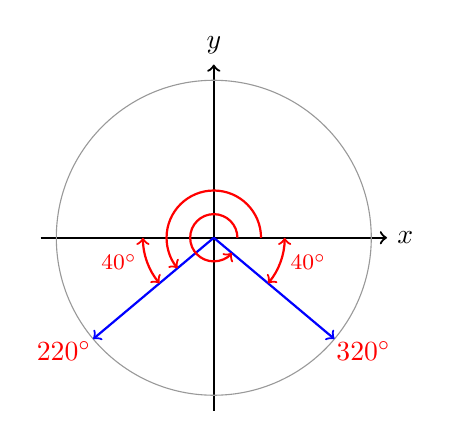
\begin{tikzpicture}
\coordinate(O) at (0,0);
\coordinate(A) at (-40:2cm);
\coordinate(B) at (220:2cm);
\draw[black, thick, ->] (0,-2.2)--(0,2.2) node[above] {$y$};
\draw[black, thick, ->] (-2.2,0)--(2.2,0) node[right] {$x$};
\draw [gray!80!white] (O) circle [radius=2cm];

\draw[blue, thick, ->] (O) -- (B) node[below left, xshift=3, yshift=3] {\color{red}$220\degree$};
\draw[blue, thick, ->] (O) -- (A) node[below right, xshift=-3, yshift=3] {\color{red}$320\degree$};

\draw [thick, red, <->] (O) ++(.9,0) arc(0:-40:.9)
   node[right, midway] {\footnotesize$40\degree$};
\draw [thick, red, <->] (O) ++(-.9,0) arc(180:220:.9)
   node[left, midway] {\footnotesize$40\degree$};
\draw [thick, red, ->] (O) ++(.3,0) arc(0:320:.3);
\draw [thick, red, ->] (O) ++(.6,0) arc(0:220:.6);

\end{tikzpicture}
\newline


exam4-1-9
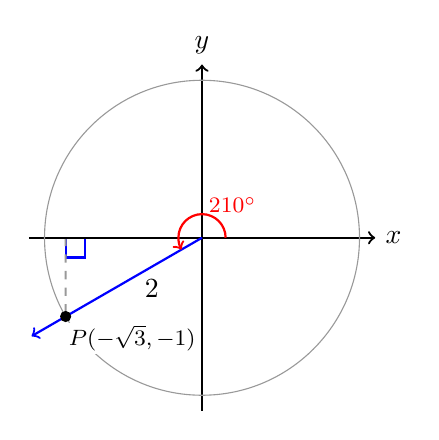
\begin{tikzpicture}
\coordinate(O) at (0,0);
\coordinate(A) at (210:2cm);
\coordinate(Ap) at (210:2.5cm);
\coordinate(B) at (-1.732,0);
\draw[blue, thick] (B) rectangle ++(.25,-.25);
\draw[gray!80!white, thick, dashed] (B)--(A);
\draw[black, thick, ->] (0,-2.2)--(0,2.2) node[above] {$y$};
\draw[black, thick, ->] (-2.2,0)--(2.2,0) node[right] {$x$};
\draw [gray!80!white] (O) circle [radius=2cm];
\draw[blue, thick, ->] (O) --(Ap);
\filldraw[black] (A) circle (1.8pt) node[anchor=north west, yshift=-2,fill=white, inner sep=1pt] {\footnotesize $P(-\sqrt{3}, -1)$};

\draw [thick, red, ->] (O) ++(.3,0) arc(0:210:.3)node[above right, midway, xshift=1, yshift=-3] {\footnotesize$210\degree$};

\node[text width=.25cm] at (-.6,-.65){ 2};

\end{tikzpicture}
\newline



fig-4-1-specang
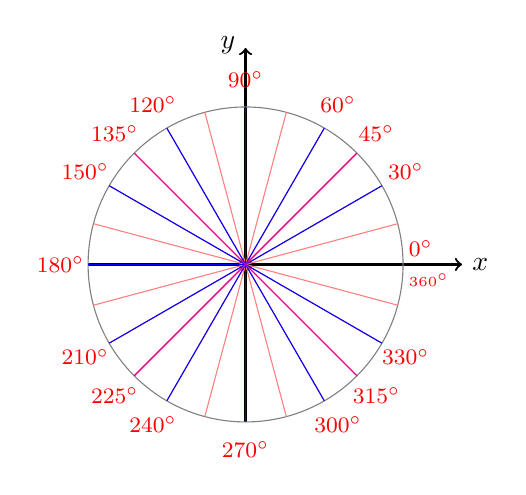
\begin{tikzpicture}
\draw[black, thick, ->] (0,-2)--(0,2.75) node[above left, yshift=-6] {$y$};
\draw[black, thick, ->] (-2,0)--(2.75,0) node[right] {$x$};

\coordinate(O) at (0,0);
\draw [gray] (O) circle [radius=2cm];
\filldraw [black] (O) circle [radius=.075cm];

\foreach \angle [count=\xi] in {15,30,...,345}
{
  \draw[red!50!white] (O) -- (\angle:2cm);
}

\foreach \angle [count=\xi] in {30,60,...,330}
{
  \draw[blue] (O) -- (\angle:2cm);
  \node[font=\footnotesize,] at (\angle:2.35cm) {$\color{red}\angle\degree$};
}

\draw[magenta] (O) -- (45:2cm);
  \node[font=\footnotesize,] at (45:2.35cm) {$\color{red}45\degree$};

\draw[magenta] (O) -- (135:2cm);
  \node[font=\footnotesize,] at (135:2.35cm) {$\color{red}135\degree$};

\draw[magenta] (O) -- (225:2cm);
  \node[font=\footnotesize,] at (225:2.35cm) {$\color{red}225\degree$};

\draw[magenta] (O) -- (315:2cm);
  \node[font=\footnotesize,] at (315:2.35cm) {$\color{red}315\degree$};

\node[text width=.25cm,font=\footnotesize] at (2.2,.2){$\color{red}\footnotesize 0\degree$ };
\node[text width=.25cm,font=\tiny] at (2.2,-.2){ $\color{red}\footnotesize 360\degree$};

\end{tikzpicture}
\newline






act4-2 grid
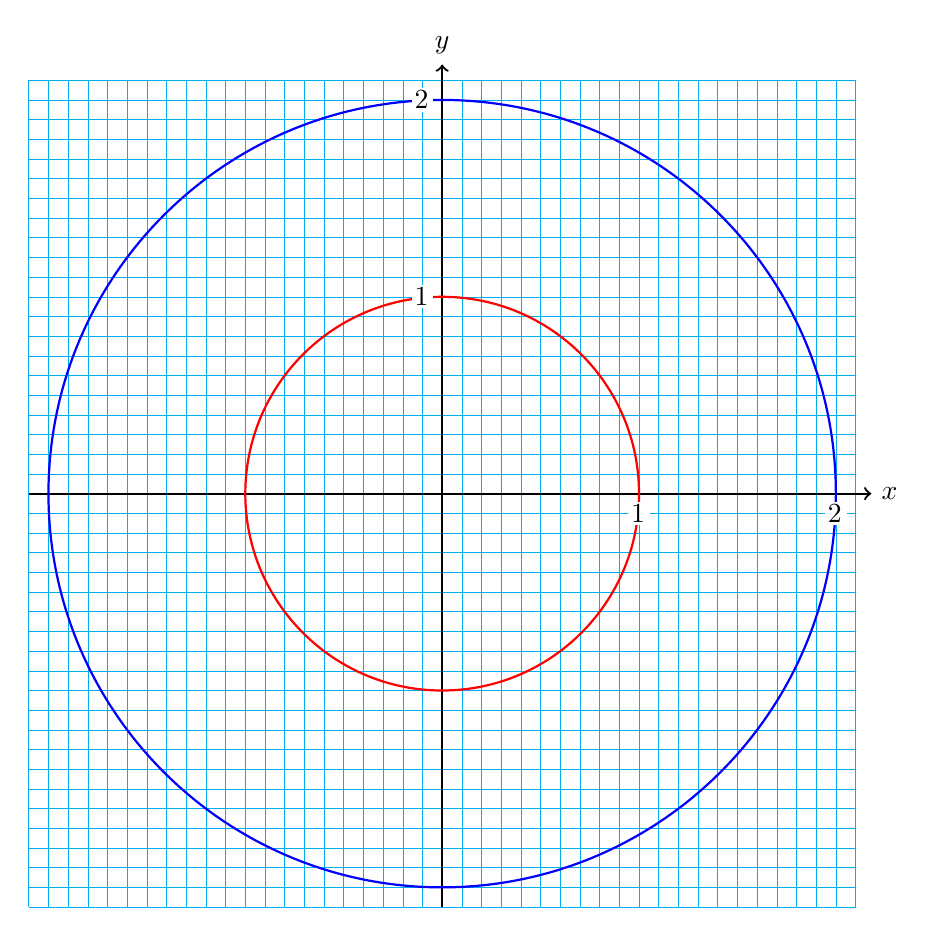
\begin{tikzpicture}[scale=.25]
\coordinate (O) at (0,0);
\draw[step=1cm,cyan,very thin] (-21,-21) grid (21,21);
\draw[thick,->] (-21,0) -- (21.8,0) node[anchor=west] {$x$};
\draw[thick,->] (0,-21) -- (0,21.8) node[anchor=south] {$y$};

\draw[red,thick] (O) circle (10);
\draw[blue,thick] (O) circle (20);

\node[text width=.2cm,fill=white,inner sep=1pt] at (10,-1)    {1};
\node[text width=.2cm,fill=white,inner sep=1pt] at (20,-1)    {2};
\node[text width=.2cm,fill=white,inner sep=1pt] at (-1,10)    {1};
\node[text width=.2cm,fill=white,inner sep=1pt] at (-1,20)    {2};
\end{tikzpicture}
\newline



act4-2 grid

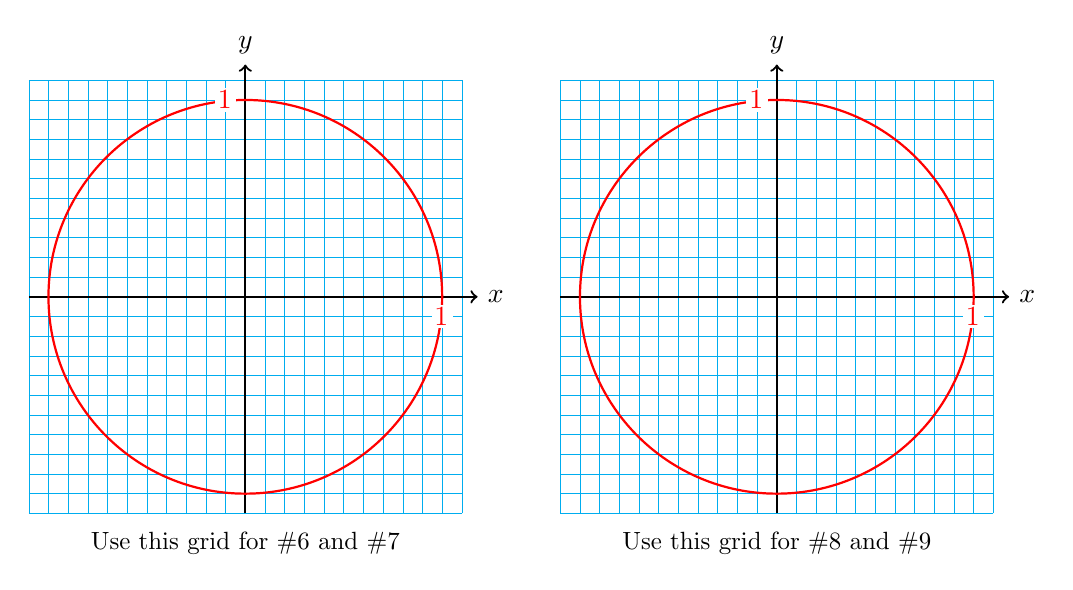
\begin{tikzpicture}[scale=.25]
\coordinate (O) at (0,0);
\draw[step=1cm,cyan,very thin] (-11,-11) grid (11,11);
\draw[thick,->] (-11,0) -- (11.8,0) node[anchor=west] {$x$};
\draw[thick,->] (0,-11) -- (0,11.8) node[anchor=south] {$y$};
\draw[red,thick] (O) circle (10);
\node[text width=.2cm,fill=white,inner sep=1pt, text=red] at (10,-1)    {1};
\node[text width=.2cm,fill=white,inner sep=1pt, text=red] at (-1,10)    {1};
\node[scale=.9] at (0,-12.5) {Use this grid for \#6 and \#7};

%second grid
\def\del{27};
\coordinate (O) at (\del,0);
\draw[step=1cm,cyan,very thin] ($ (\del,0)+(-11,-11)$) grid ($ (\del,0)+(11,11)$);
\draw[thick,->] ($ (\del,0)+(-11,0)$) --++(22.8,0) node[anchor=west] {$x$};
\draw[thick,->] ($ (\del,0)+(0,-11)$) --++(0,22.8) node[anchor=south] {$y$};
\draw[red,thick] (O) circle (10);
\node[text width=.2cm,fill=white,inner sep=1pt, text=red] at ($ (\del,0)+(10,-1) $)   {1};
\node[text width=.2cm,fill=white,inner sep=1pt, text=red] at ($ (\del,0)+(-1,10) $)   {1};
\node[scale=.9] at ($ (\del,0)+(0,-12.5)$) {Use this grid for \#8 and \#9};

\end{tikzpicture}
\newline





fig-4-1-circle2
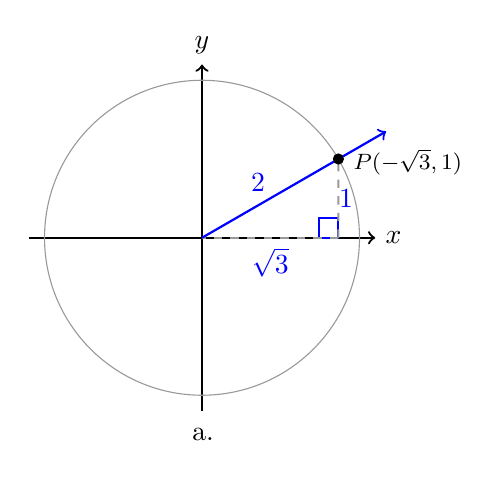
\begin{tikzpicture}
\coordinate(O) at (0,0);
\coordinate(A) at (30:2cm);
\coordinate(Ap) at (30:2.7cm);
\coordinate(B) at ($ 2* cos(30)*(1,0) $);

\draw[black, thick, ->] (0,-2.2)--(0,2.2) node[above] {$y$};
\draw[black, thick, ->] (-2.2,0)--(2.2,0) node[right] {$x$};
\draw [gray!80!white] (O) circle [radius=2cm];

\draw[blue, thick] (B) rectangle ++(-.25,.25);
\draw[gray!80!white, thick, dashed] (B)--(A) node[right, midway, xshift=-3.5]{\color{blue}1};
\draw[gray!80!white, thick, dashed] (B)--(O) node[below, midway]{\color{blue}$\sqrt{3}$};
\draw[blue, thick, ->] (O) --(Ap);
\filldraw[black] (A) circle (1.8pt) node[anchor=north west, xshift=2,yshift=7] {\footnotesize $P(-\sqrt{3}, 1)$};

\node[text width=.15cm] at (.7,.7){\color{blue} 2};
\node[text width=.25cm] at (0,-2.5){ a.};

\end{tikzpicture}
\newline


fig-4-1-unitcircle
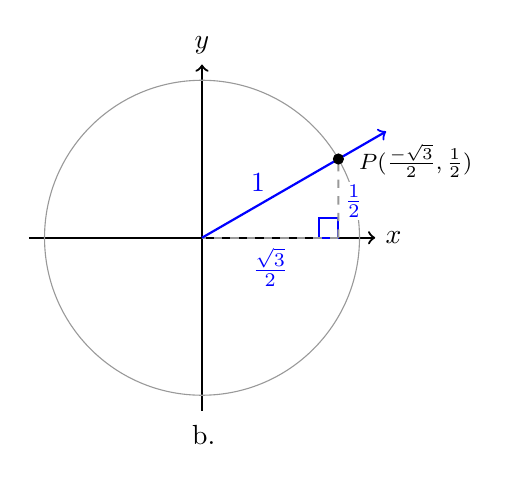
\begin{tikzpicture}
\coordinate(O) at (0,0);
\coordinate(A) at (30:2cm);
\coordinate(Ap) at (30:2.7cm);
\coordinate(B) at ($ 2* cos(30)*(1,0) $);

\draw[black, thick, ->] (0,-2.2)--(0,2.2) node[above] {$y$};
\draw[black, thick, ->] (-2.2,0)--(2.2,0) node[right] {$x$};
\draw [gray!80!white] (O) circle [radius=2cm];

\draw[blue, thick] (B) rectangle ++(-.25,.25);
\draw[gray!80!white, thick, dashed] (B)--(A) node[right, midway, xshift=1, yshift=-1,fill=white, inner sep=1pt]{\color{blue} $\frac{1}{2}  $ };
\draw[gray!80!white, thick, dashed] (B)--(O) node[below, midway]{\color{blue}$\frac{\sqrt{3}}{2}$};
\draw[blue, thick, ->] (O) --(Ap);
\filldraw[black] (A) circle (1.8pt) node[anchor=north west, xshift=4,yshift=9] {\footnotesize 
$P(\frac{-\sqrt{3}}{2}, \frac{1}{2})$};

\node[text width=.15cm] at (.7,.7){\color{blue} 1};
\node[text width=.25cm] at (0,-2.5){ b.};

\end{tikzpicture}
\newline


exam4-1-10
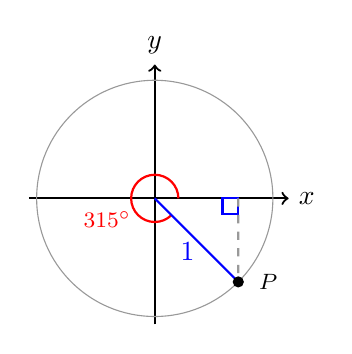
\begin{tikzpicture}
\coordinate(O) at (0,0);
\coordinate(A) at (315:1.5cm);
\coordinate(B) at ($ 1.5* cos(45)*(1,0) $);

\draw[black, thick, ->] (0,-1.6)--(0,1.7) node[above] {$y$};
\draw[black, thick, ->] (-1.6,0)--(1.7,0) node[right] {$x$};
\draw[blue,thick] (B) rectangle ++(-.2,-.2);
\draw [gray!80!white] (O) circle [radius=1.5cm];
\draw[red, thick] (.3,0) arc(0:315:0.3) node[left, midway, xshift=3, yshift=-11]{\footnotesize$315\degree$};

\draw[gray!80!white, thick, dashed] (B)--(A);
\draw[blue, thick] (O) --(A) node[left,midway, xshift=3, yshift=-4]{1};
\filldraw[black] (A) circle (1.8pt) node[anchor= west, xshift=4,yshift=0] {\footnotesize 
$P$};



\end{tikzpicture}
\newline


exer4-1-10
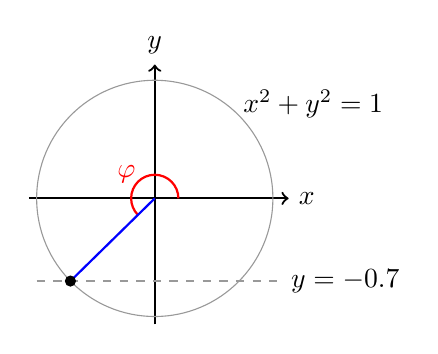
\begin{tikzpicture}
\coordinate(O) at (0,0);
\coordinate(A) at (224.43:1.5cm);
\coordinate(B) at (-1.5,-1.05);

\draw[black, thick, ->] (0,-1.6)--(0,1.7) node[above] {$y$};
\draw[black, thick, ->] (-1.6,0)--(1.7,0) node[right] {$x$};
\draw [gray!80!white] (O) circle [radius=1.5cm];
\draw[red, thick] (.3,0) arc(0:180+asin(.7):0.3) node[left, midway, xshift=0, yshift=1]{$\varphi$};

\draw[gray!80!white, thick, dashed] (B)--++(3.1,0) node[right]{{\color{black}$y=-0.7$}};
\draw[blue, thick] (O) --(A);
\filldraw[black] (A) circle (1.8pt);

\node[text width=2cm,anchor=west] at (1,1.2){ $x^2+y^2=1 $ };

\end{tikzpicture}
\newline


ar4-1-2a
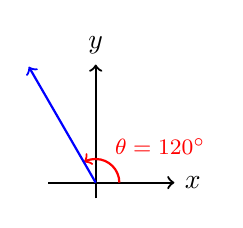
\begin{tikzpicture}
\coordinate(O) at (0,0);
\coordinate(A) at (120:1.7cm);

\draw[black, thick, ->] (0,-.2)--(0,1.5) node[above] {$y$};
\draw[black, thick, ->] (-.6,0)--(1,0) node[right] {$x$};
\draw[red, thick, ->] (.3,0) arc(0:120:0.3) node[above right, midway, xshift=-1, yshift=-1]{\footnotesize$\theta = 120\degree$};

\draw[blue, thick, ->] (O) --(A);

\end{tikzpicture}
\newline


ar4-1-2b
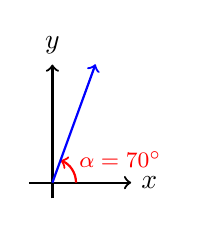
\begin{tikzpicture}
\coordinate(O) at (0,0);
\coordinate(A) at (70:1.6cm);

\draw[black, thick, ->] (0,-.2)--(0,1.5) node[above] {$y$};
\draw[black, thick, ->] (-.3,0)--(1,0) node[right] {$x$};
\draw[red, thick, ->] (.3,0) arc(0:70:0.3) node[above right, midway, xshift=-1, yshift=-3]{\footnotesize$\alpha = 70\degree$};

\draw[blue, thick, ->] (O) --(A);

\end{tikzpicture}
\newline


ar4-1-5
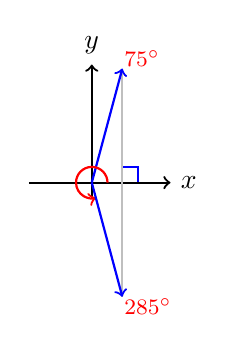
\begin{tikzpicture}
\coordinate(O) at (0,0);
\coordinate(A) at (285:1.5cm);
\coordinate(B) at (75:1.5cm);
\coordinate(C) at ($ 1.5*cos(75)*(1,0)   $);

\draw[blue,thick] (C) rectangle ++(.2,.2);
\draw[black, thick, ->] (0,-.2)--(0,1.5) node[above] {$y$};
\draw[black, thick, ->] (-.8,0)--(1,0) node[right] {$x$};

\draw[gray!50!white, thick] (A) -- (B);

\draw[blue, thick, ->] (O) --(B) node[above right,xshift=-3, yshift=-3] {\color{red}\footnotesize$75\degree$};

\draw[red, thick, ->] (.2,0) arc(0:285:0.2);

\draw[blue, thick, ->] (O) --(A) node[below right,xshift=-3, yshift=3] {\color{red}\footnotesize$285\degree$};

\end{tikzpicture}
\newline


fig-4-1-concept6
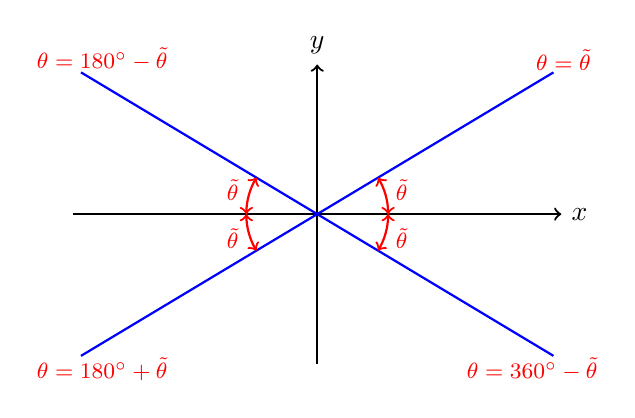
\begin{tikzpicture}

\coordinate (O) at (0,0);
\coordinate (A) at (3,1.8);
\coordinate (B) at (-3.,1.8);
\coordinate (C) at (-3,-1.8);
\coordinate (D) at (3,-1.8);

\draw[black,  thick, ->] (-3.1,0) --  (3.1,0) node[right] {$x$} ;
\draw[black,  thick, ->] (0,-1.9) --  (0,1.9) node[above] {$y$}  ;

\draw[blue, thick] (O)--(A) node[above right, xshift=-10, yshift=-3]{\footnotesize\color{red}$\theta = \tilde\theta$} ;
\draw[red, thick, <->] (.9,0) arc (0:{atan(.6)}:.9) node [right, midway,xshift=0,yshift=2] {\footnotesize$\tilde\theta$};

\draw[blue, thick] (O)--(B) node[above left, xshift=35, yshift=-3]{\footnotesize\color{red}$\theta = 180\degree- \tilde\theta$} ;
\draw[red, thick, <->] (-.9,0) arc (180:{180-atan(.6)}:.9) node [left, midway,xshift=0,yshift=2] {\footnotesize$\tilde\theta$};

\draw[blue, thick] (O)--(C) node[below left, xshift=35, yshift=3]{\footnotesize\color{red}$\theta = 180\degree + \tilde\theta$} ;
\draw[red, thick, <->] (-.9,0) arc (180:{180+atan(.6)}:.9) node [left, midway,xshift=0,yshift=-2] {\footnotesize$\tilde\theta$};

\draw[blue, thick] (O)--(D) node[below right, xshift=-35, yshift=3]{\footnotesize\color{red}$\theta = 360\degree - \tilde\theta$} ;
\draw[red, thick, <->] (.9,0) arc (0:{-atan(.6)}:.9) node [right, midway,xshift=0,yshift=-2] {\footnotesize$\tilde\theta$};

\end{tikzpicture}
\newline


hp4-1-7
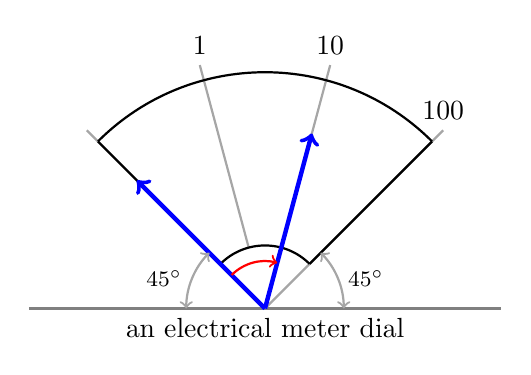
\begin{tikzpicture}

\coordinate (O) at (0,0);
\coordinate (A) at (135:3);
\coordinate (B) at (105:3);
\coordinate (C) at (75:3);
\coordinate (D) at (135:.8);
\coordinate (E) at (105:.8);
\coordinate (F) at (75:.8);
\coordinate (G) at (45:3);
\coordinate (H) at (45:.8);

\draw[gray, thick] (-3,0) --  (3,0) node[below, midway, color=black] {an electrical meter dial} ;
\draw[gray!70!white, thick] (A) --(135:3.2);
\draw[gray!70!white, thick] (E) --(105:3.2) node[above] {\color{black} 1}  ;
\draw[gray!70!white, thick] (O) --(75:3.2) node[above] {\color{black} 10}  ;
\draw[gray!70!white, thick] (O) --(45:3.2) node[above] {\color{black} 100}  ;

\draw[black,thick] (A) -- (D);
\draw[black,thick] (G) -- (H);
\draw[black,thick] (A) arc (135:45:3);
\draw[black,thick] (D) arc (135:45:.8);


\draw[blue, ultra thick, ->] (O)--(135:2.3);
\draw[blue, ultra thick, ->] (O)--(75:2.3);
\draw[red, thick, ->] (135:.6) arc (135:75:.6);

\draw[gray!70!white, thick,<->] (180:1) arc (180:135:1) node[ left, midway, xshift=0, yshift=0]{\footnotesize\color{black}$45\degree$} ;
\draw[gray!70!white, thick,<->] (1,0) arc (0:45:1) node[ right, midway, xshift=0, yshift=0]{\footnotesize\color{black}$ 45\degree$} ;

\end{tikzpicture}
\newline


hp4-1-8
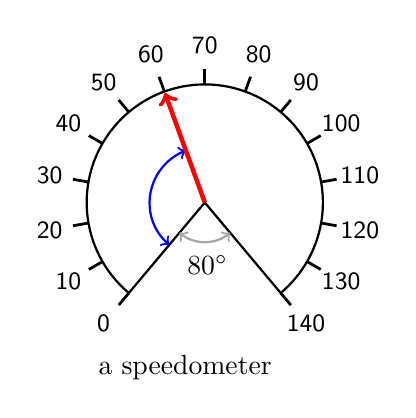
\begin{tikzpicture}
\coordinate(O) at (0,0);
\draw [black,thick] (O) -- (230:1.5) arc (230:-50:1.5) -- (O);

\foreach \angle [evaluate=\angle as \xi using int( 115 - \angle /2)] in {230,210,...,-50}
{
  \draw[line width=1pt] (\angle:1.5cm) -- (\angle:1.7cm);
  \node[font=\small] at (\angle:2cm) {\textsf{\xi}};
}

\draw[blue,thick,<->] (230:.7) arc(230:110:.7);

\draw [thick, gray!70!white, <->] (230:.5) arc (230:310:.5) node[below, midway, xshift=1, yshift=-1, color=black]{$\footnotesize 80\degree$};

\draw[red,ultra thick,->] (O) -- (110:1.48cm);

\node[text width=2.7cm] at (0,-2.1)  {a speedometer};

\end{tikzpicture}
\newline


hp4-1-9
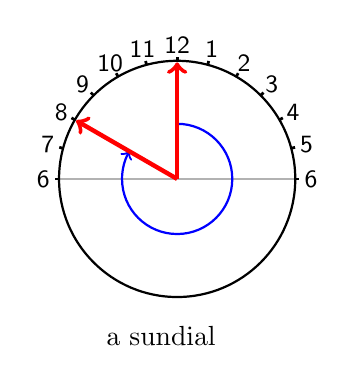
\begin{tikzpicture}
\coordinate(O) at (0,0);
\draw [gray!60!white,thick] (-1.5,0) -- (1.5,0);
\draw [black, thick] (O) circle (1.5);

\foreach \angle [count=\xi][evaluate=\xi as \xj using int( \xi+5)] in {180,165,...,90}
{
  \draw[line width=1pt] (\angle:1.5cm) -- (\angle:1.55cm);
  \node[font=\small] at (\angle:1.7cm) {\textsf{\xj}};
}
\foreach \angle [count=\xi] in {75,60,...,0}
{
  \draw[line width=1pt] (\angle:1.5cm) -- (\angle:1.55cm);
  \node[font=\small] at (\angle:1.7cm) {\textsf{\xi}};
}

\draw[blue,thick,->] (90:.7) arc(90:-210:.7);

\draw[red,ultra thick,->] (O) -- (90:1.48cm);
\draw[red,ultra thick,->] (O) -- (150:1.48cm);

\node[text width=1.8cm] at (0,-2.)  {a sundial};

\end{tikzpicture}
\newline


hp4-1-10
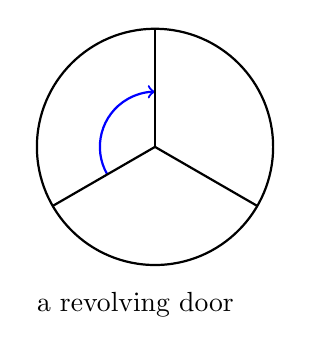
\begin{tikzpicture}
\coordinate(O) at (0,0);

\draw [black, thick] (O) circle (1.5);


\draw[blue,thick,->] (210:.7) arc(210:90:.7);

\draw[black, thick] (O) -- (90:1.5);
\draw[black, thick] (O) -- (210:1.5);
\draw[black, thick] (O) -- (-30:1.5);

\node[text width=3cm] at (0,-2.)  {a revolving door};

\end{tikzpicture}
\newline


hp4-1-11
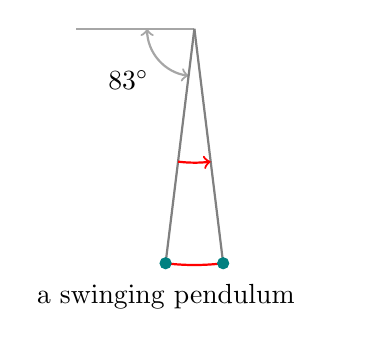
\begin{tikzpicture}
\coordinate(O) at (0,0);
\coordinate(A) at (263:3cm);
\coordinate(B) at (277:3cm);
\draw[gray!70!white, thick] (O) -- +(-1.5,0);
\draw[gray!70!white, thick, <->] (-0.6,0) arc (180: 263: .6) node[below left, midway, text=black] {$\footnotesize 83\degree$};
\draw[gray, thick] (O) -- (A);
\draw[gray, thick] (O) -- (B);

\draw [red, thick, ->] (263:1.7cm) arc (263:277:1.7);
\draw [red, thick] (263:3cm) arc (263:277:3);
\filldraw[teal] (A) circle(2pt);
\filldraw[teal] (B) circle(2pt);

\node[text width=4.cm] at (0,-3.4)  {a swinging pendulum};

\end{tikzpicture}
\newline


hp4-1-12
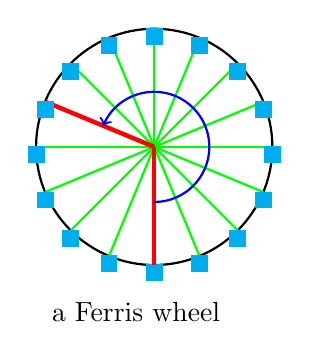
\begin{tikzpicture}
\coordinate(O) at (0,0);
\draw [black,thick] (O) circle (1.5cm) -- (O);

\foreach \angle in {0,22.5,...,337.5}
{
  \draw[green, thick] (O) -- (\angle: 1.5cm);
  \filldraw[cyan] (\angle:1.5cm)++(-.1,0) rectangle +(.2,-.2);
}

\draw[red,ultra thick] (O) -- (157.5:1.5cm);
  \filldraw[cyan] (157.5:1.5cm)++(-.1,0) rectangle +(.2,-.2);
\draw[red,ultra thick] (O) -- (-90:1.5cm);

\draw[blue,thick,->] (-90:.7) arc(-90:157.5:.7);

\node[text width=2.6cm] at (0,-2.1)  {a Ferris wheel};

\end{tikzpicture}
\newline


hp4-1-25ans
\begin{tikzpicture}
\coordinate(O) at (0,0);
\coordinate(A) at (80:1.6cm);
\coordinate(B) at (100:1.6cm);
\coordinate(C) at ($ 1.6*cos(100)*(1,0) $);

\draw[black, thick, ->] (0,-.3)--(0,1.6) node[above] {$y$};
\draw[black, thick, ->] (-.7,0)--(1.3,0) node[right] {$x$};
\draw[red, thick, ->] (.3,0) arc(0:100:0.3) node[above right, midway, xshift=-2, yshift=-4]{\footnotesize$100\degree$};
\draw[red, thick, ->] (1.1,0) arc(0:80:1.1) node[above right, midway, xshift=-1, yshift=-3]{\footnotesize$80\degree$};

\draw[gray!80!white, thick] (O) --(A);
\draw[gray!80!white,thick] (C) rectangle ++(-.16,.16); 
\draw[blue, thick] (O) --(B) -- (C)--(O);

\end{tikzpicture}
\newline


hp4-1-27ans
\begin{tikzpicture}
\coordinate(O) at (0,0);
\coordinate(A) at (36:1.6cm);
\coordinate(B) at (216:1.6cm);
\coordinate(C) at ($ 1.6*cos(216)*(1,0) $);

\draw[black, thick, ->] (0,-1.3)--(0,1.1) node[above] {$y$};
\draw[black, thick, ->] (-1.7,0)--(1.7,0) node[right] {$x$};
\draw[red, thick, ->] (.3,0) arc(0:216:0.3) node[above left, midway, xshift=2, yshift=-4]{\footnotesize$216\degree$};
\draw[red, thick, ->] (1.1,0) arc(0:36:1.1) node[above right, midway, xshift=-1, yshift=-3]{\footnotesize$36\degree$};

\draw[gray!80!white, thick] (O) --(A);
\draw[gray!80!white,thick] (C) rectangle ++(.16,-.16);
\draw[blue, thick] (O) --(B) -- (C)--(O);
\end{tikzpicture}
\newline


hp4-1-29ans
\begin{tikzpicture}
\coordinate(O) at (0,0);
\coordinate(A) at (63:1.6cm);
\coordinate(B) at (297:1.6cm);
\coordinate(C) at ($ 1.6*cos(297)*(1,0) $);

\draw[black, thick, ->] (0,-1.5)--(0,1.7) node[above] {$y$};
\draw[black, thick, ->] (-1.,0)--(1.7,0) node[right] {$x$};
\draw[red, thick, ->] (.2,0) arc(0:297:0.2) node[above left, midway, xshift=4, yshift=-1]{\footnotesize$297\degree$};
\draw[red, thick, ->] (.5,0) arc(0:63:.5) node[above right, midway, xshift=-1, yshift=-3]{\footnotesize$63\degree$};

\draw[gray!80!white, thick] (O) --(A);
\draw[gray!80!white,thick] (C) rectangle ++(-.16,-.16);
\draw[blue, thick] (O) --(B) -- (C)--(O);
\end{tikzpicture}
\newline


hp4-1-31ans
\begin{tikzpicture}
\coordinate(O) at (0,0);
\coordinate(A) at (15:1.6cm);
\coordinate(B) at (165:1.6cm);
\coordinate(C) at (195:1.6cm);
\coordinate(D) at (345:1.6cm);

\draw[black, thick, ->] (0,-1.)--(0,1.1) node[above] {$y$};
\draw[black, thick, ->] (-1.6,0)--(1.7,0) node[right] {$x$};
\draw[red, thick, ->] (.25,0) arc(0:345:0.25) node[below, midway, xshift=3, yshift=-10,fill=white, inner sep=0pt]{\footnotesize$345\degree$};
\draw[red, thick, ->] (.45,0) arc(0:195:.45) node[left,  xshift=-6, yshift=3,fill=white, inner sep=0pt]{\footnotesize$195\degree$};
\draw[red, thick, ->] (.6,0) arc(0:165:.6) node[left, midway, xshift=-6, yshift=3]{\footnotesize$165\degree$};
\draw[red, thick, ->] (.9,0) arc(0:15:.9) node[right, midway, xshift=1, yshift=1]{\footnotesize$15\degree$};

\draw[gray!80!white, thick] (O) --(A);
\draw[gray!80!white, thick] (O) --(B);
\draw[gray!80!white, thick] (O) --(C);
\draw[gray!80!white, thick] (O) --(D);
\end{tikzpicture}
\newline


hp4-1-33ans
\begin{tikzpicture}
\coordinate(O) at (0,0);
\coordinate(A) at (40:1.6cm);
\coordinate(B) at (140:1.6cm);
\coordinate(C) at (220:1.6cm);
\coordinate(D) at (320:1.6cm);

\draw[black, thick, ->] (0,-1.)--(0,1.2) node[above] {$y$};
\draw[black, thick, ->] (-1.6,0)--(1.7,0) node[right] {$x$};
\draw[red, thick, ->] (.25,0) arc(0:320:0.25) node[below, midway, xshift=7, yshift=-12,fill=white, inner sep=0pt]{\footnotesize$320\degree$};
\draw[red, thick, ->] (.45,0) arc(0:220:.45) node[left,  xshift=-4, yshift=3,fill=white, inner sep=0pt]{\footnotesize$220\degree$};
\draw[red, thick, ->] (.6,0) arc(0:140:.6) node[left, midway, xshift=0, yshift=7,fill=white, inner sep=0pt]{\footnotesize$140\degree$};
\draw[red, thick, ->] (.9,0) arc(0:40:.9) node[right, midway, xshift=1, yshift=1]{\footnotesize$40\degree$};

\draw[gray!80!white, thick] (O) --(A);
\draw[gray!80!white, thick] (O) --(B);
\draw[gray!80!white, thick] (O) --(C);
\draw[gray!80!white, thick] (O) --(D);
\end{tikzpicture}
\newline



hp4-1-35ans
\begin{tikzpicture}
\coordinate(O) at (0,0);
\coordinate(A) at (68:1.6cm);
\coordinate(B) at (112:1.6cm);
\coordinate(C) at (248:1.6cm);
\coordinate(D) at (292:1.6cm);

\draw[black, thick, ->] (0,-1.5)--(0,1.6) node[above] {$y$};
\draw[black, thick, ->] (-1.6,0)--(1.7,0) node[right] {$x$};
\draw[red, thick, ->] (.25,0) arc(0:292:0.25) node[below,  xshift=-2, yshift=-14,fill=white, inner sep=0pt]{\footnotesize$292\degree$};
\draw[red, thick, ->] (.45,0) arc(0:248:.45) node[left, midway,  xshift=-5, yshift=-2,fill=white, inner sep=0pt]{\footnotesize$248\degree$};
\draw[red, thick, ->] (.6,0) arc(0:112:.6) node[left, midway, xshift=0, yshift=10,fill=white, inner sep=0pt]{\footnotesize$112\degree$};
\draw[red, thick, ->] (.9,0) arc(0:68:.9) node[right, midway, xshift=1, yshift=1]{\footnotesize$68\degree$};

\draw[gray!80!white, thick] (O) --(A);
\draw[gray!80!white, thick] (O) --(B);
\draw[gray!80!white, thick] (O) --(C);
\draw[gray!80!white, thick] (O) --(D);
\end{tikzpicture}
\newline


hp4-1-45
\begin{tikzpicture} [scale = 1.5]
\coordinate(O) at (0,0);
\draw [black,thick] (O) circle (1.5cm) ;

\foreach \angle in {0,90,...,270}
{
  \draw[gray, thick] (O) -- (\angle: 1.5cm);
  \node[font=\small, text=blue] at (\angle:1.8cm) {$\angle\degree$};
}
\foreach \angle in {30,45,...,60}
{
  \draw[gray, thick] (O) -- (\angle: 1.5cm);
  \node[font=\small, text=blue] at (\angle:1.8cm) {$\angle\degree$};
}

\draw[gray, thick] (O) -- (120: 1.5cm);
\node[font=\small, text=blue] at (120:1.7cm) {a};
\draw[gray, thick] (O) -- (135: 1.5cm);
\node[font=\small, text=blue] at (135:1.7cm) {b};
\draw[gray, thick] (O) -- (150: 1.5cm);
\node[font=\small, text=blue] at (150:1.7cm) {c};

\draw[gray, thick] (O) -- (210: 1.5cm);
\node[font=\small, text=blue] at (210:1.7cm) {d};
\draw[gray, thick] (O) -- (225: 1.5cm);
\node[font=\small, text=blue] at (225:1.7cm) {e};
\draw[gray, thick] (O) -- (240: 1.5cm);
\node[font=\small, text=blue] at (240:1.7cm) {f};

\draw[gray, thick] (O) -- (300: 1.5cm);
\node[font=\small, text=blue] at (300:1.7cm) {g};
\draw[gray, thick] (O) -- (315: 1.5cm);
\node[font=\small, text=blue] at (315:1.7cm) {h};
\draw[gray, thick] (O) -- (330: 1.5cm);
\node[font=\small, text=blue] at (330:1.7cm) {i};

\end{tikzpicture}
\newline



hp4-1-47ans
\begin{tikzpicture}
\coordinate(O) at (0,0);
\coordinate(B) at (120:1.6cm);
\coordinate(C) at (240:1.6cm);
\coordinate(D) at (300:1.6cm);

\draw[black, thick, ->] (0,-1.5)--(0,1.6) node[above] {$y$};
\draw[black, thick, ->] (-1.6,0)--(1.7,0) node[right] {$x$};
\draw[red, thick, ->] (.25,0) arc(0:300:0.25) node[below,  xshift=-2, yshift=-14,fill=white, inner sep=0pt]{\footnotesize$300\degree$};
\draw[red, thick, ->] (.45,0) arc(0:240:.45) node[left, midway,  xshift=-5, yshift=-2,fill=white, inner sep=0pt]{\footnotesize$240\degree$};
\draw[red, thick, ->] (.6,0) arc(0:120:.6) node[left, midway, xshift=12, yshift=8,fill=white, inner sep=0pt]{\footnotesize$120\degree$};

\draw[gray!80!white, thick] (O) --(B);
\draw[gray!80!white, thick] (O) --(C);
\draw[gray!80!white, thick] (O) --(D);
\end{tikzpicture}
\newline


hp4-1-49ans
\begin{tikzpicture}
\coordinate(O) at (0,0);
\coordinate(B) at (135:1.6cm);
\coordinate(C) at (225:1.6cm);
\coordinate(D) at (315:1.6cm);

\draw[black, thick, ->] (0,-1.5)--(0,1.6) node[above] {$y$};
\draw[black, thick, ->] (-1.6,0)--(1.7,0) node[right] {$x$};
\draw[red, thick, ->] (.25,0) arc(0:315:0.25) node[below,  xshift=-2, yshift=-8,fill=white, inner sep=0pt]{\footnotesize$315\degree$};
\draw[red, thick, ->] (.45,0) arc(0:225:.45) node[left,   xshift=-7, yshift=2,fill=white, inner sep=0pt]{\footnotesize$225\degree$};
\draw[red, thick, ->] (.6,0) arc(0:135:.6) node[left, midway, xshift=14, yshift=6,fill=white, inner sep=0pt]{\footnotesize$135\degree$};

\draw[gray!80!white, thick] (O) --(B);
\draw[gray!80!white, thick] (O) --(C);
\draw[gray!80!white, thick] (O) --(D);
\end{tikzpicture}
\newline


hp4-1-73
\begin{tikzpicture}
\coordinate(O) at (0,0);
\coordinate(A) at (135:2cm);

\draw[gray!80!white, thick] (O) circle (2cm);

\draw[black, thick, ->] (0,-2.2)--(0,2.3) node[above] {$y$};
\draw[black, thick, ->] (-2.3,0)--(2.3,0) node[right] {$x$};
\draw[red, thick, ->] (.5,0) arc(0:135:0.5) node[above right, midway,  xshift=3, yshift=0,fill=white, inner sep=0pt]{\footnotesize$135\degree$};

\draw[blue, thick] (O) --(A) node[below left, midway, yshift=2] {4};
\filldraw[red] (A) circle (2pt);
\end{tikzpicture}
\newline


hp4-1-74
\begin{tikzpicture}
\coordinate(O) at (0,0);
\coordinate(A) at (300:2cm);

\draw[gray!80!white, thick] (O) circle (2cm);

\draw[black, thick, ->] (0,-2.2)--(0,2.3) node[above] {$y$};
\draw[black, thick, ->] (-2.3,0)--(2.3,0) node[right] {$x$};
\draw[red, thick, ->] (.5,0) arc(0:300:0.5) node[above left, midway,  xshift=-1, yshift=0,fill=white, inner sep=0pt]{\footnotesize$300\degree$};

\draw[blue, thick] (O) --(A) node[above right, midway, yshift=-2] {6};
\filldraw[red] (A) circle (2pt);
\end{tikzpicture}
\newline


hp4-1-75
\begin{tikzpicture}
\coordinate(O) at (0,0);
\coordinate(A) at (60:2cm);

\draw[gray!80!white, thick] (O) circle (2cm);

\draw[black, thick, ->] (0,-2.2)--(0,2.3) node[above] {$y$};
\draw[black, thick, ->] (-2.3,0)--(2.3,0) node[right] {$x$};
\draw[red, thick, ->] (.5,0) arc(0:60:0.5) node[right, midway,  xshift=0, yshift=0]{\footnotesize$60\degree$};

\draw[blue, thick] (O) --(A) node[above left, midway, yshift=-2] {3};
\filldraw[red] (A) circle (2pt);
\end{tikzpicture}
\newline


hp4-1-76
\begin{tikzpicture}
\coordinate(O) at (0,0);
\coordinate(A) at (30:2cm);

\draw[gray!80!white, thick] (O) circle (2cm);

\draw[black, thick, ->] (0,-2.2)--(0,2.3) node[above] {$y$};
\draw[black, thick, ->] (-2.3,0)--(2.3,0) node[right] {$x$};
\draw[red, thick, ->] (.7,0) arc(0:30:0.7) node[right, midway,  xshift=0, yshift=0]{\footnotesize$30\degree$};

\draw[blue, thick] (O) --(A) node[above left, midway, xshift=2, yshift=-2] {12};
\filldraw[red] (A) circle (2pt);
\end{tikzpicture}
\newline


hp4-1-77
\begin{tikzpicture}
\coordinate(O) at (0,0);
\coordinate(A) at (210:2cm);

\draw[gray!80!white, thick] (O) circle (2cm);

\draw[black, thick, ->] (0,-2.2)--(0,2.3) node[above] {$y$};
\draw[black, thick, ->] (-2.3,0)--(2.3,0) node[right] {$x$};
\draw[red, thick, ->] (.5,0) arc(0:210:0.5) node[above left, midway,  xshift=0, yshift=-3]{\footnotesize$210\degree$};

\draw[blue, thick] (O) --(A) node[below right, midway, xshift=-2, yshift=2] {1};
\filldraw[red] (A) circle (2pt);
\end{tikzpicture}
\newline


hp4-1-78
\begin{tikzpicture}
\coordinate(O) at (0,0);
\coordinate(A) at (225:2cm);

\draw[gray!80!white, thick] (O) circle (2cm);

\draw[black, thick, ->] (0,-2.2)--(0,2.3) node[above] {$y$};
\draw[black, thick, ->] (-2.3,0)--(2.3,0) node[right] {$x$};
\draw[red, thick, ->] (.5,0) arc(0:225:0.5) node[above left, midway,  xshift=0, yshift=-3]{\footnotesize$225\degree$};

\draw[blue, thick] (O) --(A) node[below right, midway, xshift=-2, yshift=2] {1};
\filldraw[red] (A) circle (2pt);
\end{tikzpicture}
\newline


hp4-1-79
\begin{tikzpicture}[scale=.25]

\coordinate (O) at (0,0);
\coordinate (P) at (200:10);
\coordinate (Q) at (200:20);

\draw[step=1cm,cyan,very thin] (-21,-21) grid (21,21);
\draw[thick,->] (-21,0) -- (21.8,0) node[anchor=west] {$x$};
\draw[thick,->] (0,-21) -- (0,21.8) node[anchor=south] {$y$};
\draw[black,  thick] (Q)++(200:2)--(O) ;

\draw[red,thick] (O) circle (10);
\draw[blue,thick] (O) circle (20);

\filldraw[red] (P) circle (.25cm) node[anchor=north east, yshift=-5,fill=white,inner sep=1pt]{$P$};
\filldraw[blue] (Q) circle (.25cm) node[anchor=north east, yshift=-5,fill=white,inner sep=1pt]{$Q$} ;

\draw[gray, thick, ->] (3,0) arc(0:200:3) node[above left,midway, xshift=0, yshift=0,fill=white,inner sep=1pt, text=black] {$\small 200\degree$};

\node[text width=.2cm,fill=white,inner sep=1pt] at (10,-1)    {1};
\node[text width=.2cm,fill=white,inner sep=1pt] at (20,-1)    {2};
\node[text width=.2cm,fill=white,inner sep=1pt] at (-1,10)    {1};
\node[text width=.2cm,fill=white,inner sep=1pt] at (-1,20)    {2};

\end{tikzpicture}
\newline


hp4-1-80
\begin{tikzpicture}[scale=.25]

\coordinate (O) at (0,0);
\coordinate (P) at (228:10);
\coordinate (Q) at (228:20);

\draw[step=1cm,cyan,very thin] (-21,-21) grid (21,21);
\draw[thick,->] (-21,0) -- (21.8,0) node[anchor=west] {$x$};
\draw[thick,->] (0,-21) -- (0,21.8) node[anchor=south] {$y$};
\draw[black,  thick] (Q)++(228:8)--(O) ;

\draw[red,thick] (O) circle (10);
\draw[blue,thick] (O) circle (20);

\filldraw[red] (P) circle (.25cm) node[anchor=north , yshift=-7,fill=white,inner sep=1pt]{$P$};
\filldraw[blue] (Q) circle (.25cm) node[anchor=north , yshift=-7,fill=white,inner sep=1pt]{$Q$} ;

\draw[gray, thick, ->] (3,0) arc(0:228:3) node[above left,midway, xshift=0, yshift=0,fill=white,inner sep=1pt, text=black] {$\small 228\degree$};

\node[text width=.2cm,fill=white,inner sep=1pt] at (10,-1)    {1};
\node[text width=.2cm,fill=white,inner sep=1pt] at (20,-1)    {2};
\node[text width=.2cm,fill=white,inner sep=1pt] at (-1,10)    {1};
\node[text width=.2cm,fill=white,inner sep=1pt] at (-1,20)    {2};

\end{tikzpicture}
\newline


hp4-1-81
\begin{tikzpicture}[scale=.25]

\coordinate (O) at (0,0);
\coordinate (P) at (160:10);
\coordinate (Q) at (160:20);

\draw[step=1cm,cyan,very thin] (-21,-21) grid (21,21);
\draw[thick,->] (-21,0) -- (21.8,0) node[anchor=west] {$x$};
\draw[thick,->] (0,-21) -- (0,21.8) node[anchor=south] {$y$};
\draw[black,  thick] (Q)++(160:2)--(O) ;

\draw[red,thick] (O) circle (10);
\draw[blue,thick] (O) circle (20);

\filldraw[red] (P) circle (.25cm) node[anchor=south east , yshift=7,fill=white,inner sep=1pt]{$P$};
\filldraw[blue] (Q) circle (.25cm) node[anchor=south east , yshift=7,fill=white,inner sep=1pt]{$Q$} ;

\draw[gray, thick, ->] (3,0) arc(0:160:3) node[above right,midway, xshift=0, yshift=0,fill=white,inner sep=1pt, text=black] {$\small 160\degree$};

\node[text width=.2cm,fill=white,inner sep=1pt] at (10,-1)    {1};
\node[text width=.2cm,fill=white,inner sep=1pt] at (20,-1)    {2};
\node[text width=.2cm,fill=white,inner sep=1pt] at (-1,10)    {1};
\node[text width=.2cm,fill=white,inner sep=1pt] at (-1,20)    {2};

\end{tikzpicture}
\newline


hp4-1-82
\begin{tikzpicture}[scale=.25]

\coordinate (O) at (0,0);
\coordinate (P) at (312:10);
\coordinate (Q) at (312:20);

\draw[step=1cm,cyan,very thin] (-21,-21) grid (21,21);
\draw[thick,->] (-21,0) -- (21.8,0) node[anchor=west] {$x$};
\draw[thick,->] (0,-21) -- (0,21.8) node[anchor=south] {$y$};
\draw[black,  thick] (Q)++(312:10)--(O) ;

\draw[red,thick] (O) circle (10);
\draw[blue,thick] (O) circle (20);

\filldraw[red] (P) circle (.25cm) node[anchor=west , xshift=7,fill=white,inner sep=1pt]{$P$};
\filldraw[blue] (Q) circle (.25cm) node[anchor=west , xshift=7,fill=white,inner sep=1pt]{$Q$} ;

\draw[gray, thick, ->] (3,0) arc(0:312:3) node[above left,midway, xshift=0, yshift=0,fill=white,inner sep=1pt, text=black] {$\small 312\degree$};

\node[text width=.2cm,fill=white,inner sep=1pt] at (10,-1)    {1};
\node[text width=.2cm,fill=white,inner sep=1pt] at (20,-1)    {2};
\node[text width=.2cm,fill=white,inner sep=1pt] at (-1,10)    {1};
\node[text width=.2cm,fill=white,inner sep=1pt] at (-1,20)    {2};

\end{tikzpicture}
\newline


\subsection{4.2 Graphs of trig functions}





fig-4-2-rcircle
\begin{tikzpicture}
\coordinate(O) at (0,0);
\coordinate(P) at (50:2cm);
\coordinate(Q) at ($ 2*cos(50)*(1,0)$);
\coordinate(R) at (50:0.9cm);
\coordinate(S) at ($ 0.9*cos(50)*(1,0)$);


\draw[gray!80!white, thick] (P) -- (Q);
\draw[gray!80!white, thick] (Q) rectangle ++(-.2,.2);
\draw[gray!80!white, thick] (R) -- (S);
\draw[gray!80!white, thick] (S) rectangle ++(-.2,.2);

\draw[black, thick] (O) circle (2cm);
\draw[black, thick] (O) circle (0.9cm);

\draw[black, thick, ->] (0,-2.2)--(0,2.3) node[above] {$y$};
\draw[black, thick, ->] (-2.3,0)--(2.3,0) node[right] {$x$};

\draw[blue, thick] (O) --(P) node[above , yshift=0] {$P$};
\filldraw[blue] (P) circle (2pt)  node[anchor=west , xshift=3] {($r \, \cos \theta, r \, \sin \theta)$};
\filldraw[blue] (R) circle (2pt);

\node[text width=2cm,fill=white, inner sep=1pt] at (0.2,-1.3)    {\small $x^2+y^2=1$};
\node[text width=2cm] at (2,-2.)    {\small
$x^2+y^2=r^2$};

\end{tikzpicture}
\newline


exam4-2-1
\begin{tikzpicture}
\coordinate(O) at (0,0);
\coordinate(P) at (292:2cm);
\coordinate(Q) at ($ 2*cos(292)*(1,0)$);
\coordinate(R) at (292:2.3cm);

\draw[gray!80!white, thick] (Q) rectangle ++(-.2,-.2);
\draw[gray!80!white, thick, dashed] (P) -- (Q);

\draw[black, thick, ->] (0,-2.2)--(0,1.3) node[above] {$y$};
\draw[black, thick, ->] (-1.5,0)--(2.3,0) node[right] {$x$};
\draw[gray!80!white, ultra thick, dashed] (Q) -- (O);

\draw[red, thick, ->] (0.25,0) arc (0:292:0.25) node[left, midway, yshift=-12] {$\scriptsize 292\degree$};
\draw[blue, thick] (O) --(R) ;
\filldraw[blue] (P) circle (2pt)  node[anchor=west , xshift=3] {$P(x,y)$};

\node[text width=1cm,fill=white, inner sep=1pt] at (0.0,-1.5)    {$\color{blue}\scriptsize r=6$};

\end{tikzpicture}
\newline


\section {Stuff for later}





Section 4.2 Angle of inclination
\begin{tikzpicture}

\coordinate (O) at (0,0);
\coordinate (x) at (3.5,0);
\coordinate (y) at (0,2);
\coordinate (A) at (3,1.8);
\coordinate (B) at (1.,0);
\coordinate (C) at (2.5,0);
\coordinate (D) at (-1,-1.8);

\draw[black,  thick, ->] (-1.5,0) --  (x) node[right] {$x$} ;
\draw[black,  thick, ->] (0,-2) --  (y) node[above] {$y$}  ;
\draw[black,  thick, <->] (D) --  (A)  ;
\draw[red, thick] (1.9,0) arc (0:{atan(0.9)}:.9) node [left, midway,xshift=0,yshift=-3] {$\alpha$};

\end{tikzpicture}
\newline



Section 4.2 Angle of inclination
\begin{tikzpicture}

\coordinate (O) at (0,0);
\coordinate (x) at (3.5,0);
\coordinate (y) at (0,2);
\coordinate (A) at (3,1.8);
\coordinate (B) at (1.,0);
\coordinate (C) at (2.5,0);
\coordinate (D) at (-1,-1.8);

\draw[black,  thick, ->] (-1.5,0) --  (x) node[right] {$x$} ;
\draw[black,  thick, ->] (0,-2) --  (y) node[above] {$y$}  ;
\draw[black,  thick, <->] (D) --  (A)  ;
\draw[red, thick] (1.9,0) arc (0:{atan(0.9)}:.9) node [left, midway,xshift=0,yshift=-3] {$\alpha$};

\draw[green, ultra thick, dashed] (1,-.03) -- (2.5,-.03);
\draw[green, ultra thick, dashed] (2.5,1.35) -- (2.5,0);

\end{tikzpicture}
\newline


On a unit circle
\begin{tikzpicture} [scale=1.7]

\draw[thick,->] (-1.2,0) -- (1.3,0) node[anchor=west] {$x$};
\draw[thick,->] (0,-1.2) -- (0,1.3) node[anchor=south] {$y$};

\coordinate(O) at (0,0);
\coordinate(A) at (1,0);
\coordinate (B) at (-.6428,0.766);

\draw[gray,thick] (O) circle (1);
\draw[blue,thick] (O) -- (B) node[below left, midway, xshift=2, yshift=4] {\small\color{blue} $r=1$};
\filldraw [blue] (A) circle (1pt);
\filldraw [blue] (B) circle (1pt);
\draw[blue,thick] (A) arc(0:130:1) node[above, midway, xshift=14, yshift=-8] {\color{blue}$s$};
\draw[red,thick] (O)++(.2,0) arc(0:130:.2) node[above, midway, xshift=4, yshift=-3] {\color{blue}$\theta$};

\end{tikzpicture}
\newline



sine graph
\begin{tikzpicture}

\draw[cyan,xstep=pi/12,ystep=0.18]
(-2*pi,-1.8) grid (2*pi,1.8);

\draw[->] (-6.3,0) -- (6.5,0) node[right] {$\theta$};
\draw[->] (0,-1.8) -- (0,2.2) node[above] {$f(\theta)=\sin(\theta)$};

\foreach \x in {-24,-23,...,24}
\draw[black] ($ pi*\x /12*(1,0) +(0,.08) $) --++(0,-.16);
\foreach \y in {-0.9, 0.9}
\draw[black] (.08,\y ) --++(-.16,0);
\foreach \y in {-1,1}
\draw[black, thick] (.12,1.8*\y ) --++(-.24,0) node[anchor=east, xshift=-3, fill=white, inner sep=1pt] {\y};

\draw[black, thick] (-2*pi,.2) --++(0,-.4) node[anchor=north, xshift=-2,yshift=-3, fill=white, inner sep=1pt] {$-2\pi$};
\draw[black, thick] (2*pi,.2) --++(0,-.4) node[anchor=north, xshift=2,yshift=-3, fill=white, inner sep=1pt] {$2\pi$};

\draw[black] (pi,.2) --++(0,-.4) node[anchor=north, yshift=-3, fill=white, inner sep=1pt] {$\pi$};

\draw[black] (pi,.2) --++(0,-.4) node[anchor=north, yshift=-3, fill=white, inner sep=1pt] {$\pi$};
\draw[black] (-pi,.2) --++(0,-.4) node[anchor=north, xshift=-2,yshift=-3, fill=white, inner sep=1pt] {$-\pi$};
\draw[black] (-pi/2,.15) --++(0,-.3) node[anchor=north, yshift=-3, fill=white, inner sep=1pt] {$\frac{-\pi}{2}$};
\draw[black] (pi/2,.15) --++(0,-.3) node[anchor=north, yshift=-3, fill=white, inner sep=1pt] {$\frac{\pi}{2}$};
\draw[black] (3*pi/2,.15) --++(0,-.3) node[anchor=north, yshift=-3, fill=white, inner sep=1pt] {$\frac{3\pi}{2}$};
\draw[black] (-3*pi/2,.15) --++(0,-.3) node[anchor=north, yshift=-3, fill=white, inner sep=1pt] {$\frac{-3\pi}{2}$};

\draw[black] (pi/4,.11) --++(0,-.22) node[anchor=north, yshift=-4, fill=white, inner sep=1pt] {$\frac{\pi}{4}$};

\draw[black] (3*pi/4,.11) --++(0,-.22) node[anchor=north, yshift=-3, fill=white, inner sep=1pt] {$\frac{3\pi}{4}$};

\draw[domain=-2*pi:2*pi,smooth,variable=\x,red,very thick] plot ({\x},{1.8*sin(deg(\x))});

\end{tikzpicture}
\newline


cosine graph
\begin{tikzpicture} 

\draw[cyan,xstep=pi/12,ystep=0.18]
(-2*pi,-1.8) grid (2*pi,1.8);

\draw[->] (-6.3,0) -- (6.5,0) node[right] {$\theta$};
\draw[->] (0,-1.8) -- (0,2.2) node[above] {$f(\theta)=\cos(\theta)$};

\foreach \x in {-24,-23,...,24}
\draw[black] ($ pi*\x /12*(1,0) +(0,.08) $) --++(0,-.16);
\foreach \y in {-0.9, 0.9}
\draw[black] (.08,\y ) --++(-.16,0);
\foreach \y in {-1,1}
\draw[black, thick] (.12,1.8*\y ) --++(-.24,0) node[anchor=east, xshift=-3, fill=white, inner sep=1pt] {\y};

\draw[black, thick] (-2*pi,.2) --++(0,-.4) node[anchor=north, xshift=-2,yshift=-3, fill=white, inner sep=1pt] {$-2\pi$};
\draw[black, thick] (2*pi,.2) --++(0,-.4) node[anchor=north, xshift=2,yshift=-3, fill=white, inner sep=1pt] {$2\pi$};

\draw[black] (pi,.2) --++(0,-.4) node[anchor=north, yshift=-3, fill=white, inner sep=1pt] {$\pi$};

\draw[black] (pi,.2) --++(0,-.4) node[anchor=north, yshift=-3, fill=white, inner sep=1pt] {$\pi$};
\draw[black] (-pi,.2) --++(0,-.4) node[anchor=north, xshift=-2,yshift=-3, fill=white, inner sep=1pt] {$-\pi$};
\draw[black] (-pi/2,.15) --++(0,-.3) node[anchor=north, yshift=-3, fill=white, inner sep=1pt] {$\frac{-\pi}{2}$};
\draw[black] (pi/2,.15) --++(0,-.3) node[anchor=north, yshift=-3, fill=white, inner sep=1pt] {$\frac{\pi}{2}$};
\draw[black] (3*pi/2,.15) --++(0,-.3) node[anchor=north,xshift=3, yshift=-3, fill=white, inner sep=1pt] {$\frac{3\pi}{2}$};
\draw[black] (-3*pi/2,.15) --++(0,-.3) node[anchor=north,xshift=-3, yshift=-3, fill=white, inner sep=1pt] {$\frac{-3\pi}{2}$};

\draw[black] (pi/4,.11) --++(0,-.22) node[anchor=north, yshift=-4, fill=white, inner sep=1pt] {$\frac{\pi}{4}$};

\draw[black] (3*pi/4,.11) --++(0,-.22) node[anchor=north, yshift=-3, fill=white, inner sep=1pt] {$\frac{3\pi}{4}$};

\draw[black] (5*pi/4,.11) --++(0,-.22) node[anchor=north, yshift=-3, fill=white, inner sep=1pt] {$\frac{5\pi}{4}$};

\draw[domain=-2*pi:2*pi,smooth,variable=\x,red,very thick] plot ({\x},{1.8*cos(deg(\x))});

\end{tikzpicture}
\newline


tangent graph
\begin{tikzpicture} [yscale=.5]

\draw[cyan,xstep=pi/12,ystep=0.5]
(-2*pi,-5) grid (2*pi,5);

\draw[->] (-6.3,0) -- (6.5,0) node[right] {$\theta$};
\draw[->] (0,-5) -- (0,5.5) node[above] {$f(\theta)=\tan(\theta)$};

\foreach \x in {-24,-23,...,24}
\draw[black] ($ pi*\x /12*(1,0) +(0,.08) $) --++(0,-.16);
\foreach \y in {-5,-4,...,-1,1,2,...,5}
\draw[black, thick] (.10,\y ) --++(-.2,0) node[anchor=east, xshift=-3, fill=white, inner sep=1pt] {\y};

\draw[black, thick] (-2*pi,.2) --++(0,-.4) node[anchor=north, xshift=-2,yshift=-3, fill=white, inner sep=1pt] {$-2\pi$};
\draw[black, thick] (2*pi,.2) --++(0,-.4) node[anchor=north, xshift=2,yshift=-3, fill=white, inner sep=1pt] {$2\pi$};

\draw[black] (pi,.2) --++(0,-.4) node[anchor=north, yshift=-3, fill=white, inner sep=1pt] {$\pi$};

\draw[black] (pi,.2) --++(0,-.4) node[anchor=north, yshift=-3, fill=white, inner sep=1pt] {$\pi$};
\draw[black] (-pi,.2) --++(0,-.4) node[anchor=north, xshift=-2,yshift=-3, fill=white, inner sep=1pt] {$-\pi$};
\draw[black] (-pi/2,.15) --++(0,-.3) node[anchor=north, yshift=-3, fill=white, inner sep=1pt] {$\frac{-\pi}{2}$};
\draw[black] (pi/2,.15) --++(0,-.3) node[anchor=north, yshift=-3, fill=white, inner sep=1pt] {$\frac{\pi}{2}$};
\draw[black] (3*pi/2,.15) --++(0,-.3) node[anchor=north,xshift=3, yshift=-3, fill=white, inner sep=1pt] {$\frac{3\pi}{2}$};
\draw[black] (-3*pi/2,.15) --++(0,-.3) node[anchor=north,xshift=-3, yshift=-3, fill=white, inner sep=1pt] {$\frac{-3\pi}{2}$};

\draw[black] (pi/4,.11) --++(0,-.22) node[anchor=north, yshift=-4, fill=white, inner sep=1pt] {$\frac{\pi}{4}$};

\draw[black] (3*pi/4,.11) --++(0,-.22) node[anchor=north, yshift=-3, fill=white, inner sep=1pt] {$\frac{3\pi}{4}$};

\draw[black] (5*pi/4,.11) --++(0,-.22) node[anchor=north, yshift=-3, fill=white, inner sep=1pt] {$\frac{5\pi}{4}$};

\foreach \i in {-1, 0, 1}
	\draw[domain={\i*pi-atan(5)*pi/180}:{\i*pi+atan(5)*pi/180}, smooth, variable=\x,red,very thick] plot ({\x},{tan(deg(\x))}) ;

\draw[domain={-2*pi:atan(5)*pi/180-2*pi}, smooth, variable=\x,red,very thick] plot ({\x},{tan(deg(\x))}) ;
\draw[domain={2*pi-atan(5)*pi/180:2*pi}, smooth, variable=\x,red,very thick] plot ({\x},{tan(deg(\x))}) ;

\end{tikzpicture}
\newline


part A: law of sines a circumscribing circle

\begin{tikzpicture} [scale=.4]

\coordinate (O) at (0,0);
\coordinate (A) at (-3,-4);
\coordinate (B) at (3,-4);
\coordinate (C) at (-1.92,4.62);

\filldraw (A) circle (.1cm) node[anchor=north east] {$A$};
\filldraw (B) circle (.1cm) node[anchor=north west] {$B$};
\filldraw (C) circle (.1cm) node[anchor=south east] {$C$};

\draw[black,thick] (A)--(B)--(C)--(A);
\draw[gray!40!white, thick, dashed](O)++(0,1) -- (0,-4)--+(0,-.5);
\draw[gray!40!white, thick, dashed](O)++(.862,-.108) -- (-2.96,.31)--++(-.862,.108);
\draw[blue!80!white,thick] (0,-4)++(.75,0)-- ++(0,.75) -- ++(-.75,0);
\draw[blue!80!white,thick] (-2.46,.31) ++(.0864,.6896) -- ++(.6896,-.0864) -- ++(-.0864,-.6896);
\filldraw (O) circle (.2cm) node[anchor=north east] {$O$};

\draw[blue] (O) circle (5);

\end{tikzpicture}
\newline

part B: law of sines a circumscribing circle

\begin{tikzpicture} [scale=.4]

\coordinate (O) at (0,0);
\coordinate (A) at (-3,-4);
\coordinate (B) at (3,-4);
\coordinate (C) at (-1.92,4.62);
\coordinate (Cp) at (-4.62,1.92);
\coordinate (Cpp) at (0,5);
\coordinate (Cppp) at (3,4);
\coordinate (Cpppp) at (5,0);

\filldraw (O) circle (.1cm) node[anchor=north east] {$O$};
\filldraw (A) circle (.1cm) node[anchor=north east] {$A$};
\filldraw (B) circle (.1cm) node[anchor=north west] {$B$};
\filldraw (C) circle (.1cm) node[anchor=south east] {$C$};

\draw[draw= blue, fill=blue!80!white] (A)--(B)--(C)--(A);
\draw[draw= blue, fill=blue!30!white, opacity=.5] (A)--(B)--(Cp)--(A);
\draw[draw= blue, fill=blue!30!white, opacity=.5] (A)--(B)--(Cpp)--(A);
\draw[draw= blue, fill=blue!30!white, opacity=.5] (A)--(B)--(Cppp)--(A);
\draw[draw= blue, fill=blue!30!white, opacity=.5] (A)--(B)--(Cpppp)--(A);


\draw[blue] (O) circle (5);

\end{tikzpicture}
\newline

Exercise not used?
\begin{tikzpicture}
\coordinate (O) at (0,0);
\coordinate (A) at (0,0);
\coordinate (B) at (0,0);
\coordinate(C) at (0,0);
\coordinate (D) at (0,0);
\filldraw[black] (O) circle (.2pt) node[anchor=south west, xshift=6]{$50\degree$};
\filldraw[black] (A) circle (.2pt) node[anchor=south east]{$x$};
\filldraw[black] (B) circle (.2pt) node[anchor=north east, xshift=-6]{$y$};
\filldraw[black] (C) circle (.2pt) node[anchor=north west]{$z$};
%\draw[black,  thick] (A) -- (B) --( C) -- cycle;
\draw[black] (-2.3,0) --  (2.3,0);
\draw[black] (0.8,1.3) --  (-0.8,-1.3) ;
\end{tikzpicture}
\newline


\end{document}
